%&pdflatex
\documentclass[12pt]{article}
\usepackage{algorithmicx}
\usepackage[ruled]{algorithm}
\usepackage{algpseudocode}
\usepackage{algpascal}
\usepackage{algc}
\usepackage{url,enumerate, amssymb, anysize, booktabs, amsfonts}
\usepackage[colorlinks = true,
linkcolor = blue,
urlcolor  = blue,
citecolor = green,
anchorcolor = blue]{hyperref}
\usepackage{setspace,listings}
\usepackage[dvipdfmx]{graphicx}
\usepackage{amsmath}
\usepackage{psfrag}
\usepackage[font=small,labelfont=bf]{caption}
\usepackage{enumerate}
\usepackage{natbib}
\usepackage{url} % not crucial - just used below for the URL 

% NOTE: To produce blinded version, replace "0" with "1" below.
\newcommand{\blind}{1}

% DON'T change margins - should be 1 inch all around.
\addtolength{\oddsidemargin}{-.5in}%
\addtolength{\evensidemargin}{-.5in}%
\addtolength{\textwidth}{1in}%
\addtolength{\textheight}{-.3in}%
\addtolength{\topmargin}{-.8in}%
\usepackage{color,amssymb}
\usepackage{fancyhdr, mathtools}
\usepackage{dcolumn}
\usepackage{indentfirst, verbatim}
%\newcounter{equationset, sectsty, breqn}
\usepackage{setspace,float,lscape,amsmath,color}
\usepackage{color,amssymb}
\usepackage{fancyhdr, mathtools, amsthm}
\theoremstyle{definition}
\newtheorem{definition}{Definition}[section]
\newtheorem{theorem}{Theorem}[section]
\newtheorem{corollary}{Corollary}[theorem]
\newtheorem{lemma}[theorem]{Lemma}
\newtheorem{remark}{Remark}


\newcommand{\Linefor}[2]{%
	\State \algorithmicfor\ {#1}\ \algorithmicdo\ {#2} \algorithmicend\ \algorithmicfor%
}
\newcommand{\Lineif}[2]{%
	\State \algorithmicif\ {#1}\ \algorithmicdo\ {#2} \algorithmicend\ \algorithmicif%
}


\renewcommand{\algorithmicrequire}{\textbf{Input:}}
\renewcommand{\algorithmicensure}{\textbf{Output:}}

%\usepackage{algorithmicx}

%\algdisablelines

\begin{document}
	
	%\bibliographystyle{natbib}
	
	\def\spacingset#1{\renewcommand{\baselinestretch}%
		{#1}\small\normalsize} \spacingset{1}
	
	
	%%%%%%%%%%%%%%%%%%%%%%%%%%%%%%%%%%%%%%%%%%%%%%%%%%%%%%%%%%%%%%%%%%%%%%%%%%%%%%
	
	\if1\blind
	{
		\title{\bf Testing independence between networks and nodal attributes via multiscale metrics}
		\author{Youjin Lee\thanks{
				The authors gratefully acknowledge \textit{please remember to list all relevant funding sources in the unblinded version}}\hspace{.2cm}\\
			Department of Biostatistics, Johns Hopkins School of Public Health\\
			and \\
			Author 2 \\
			Department of ZZZ, University of WWW}
		\maketitle
	} \fi
	
	\if0\blind
	{
		\bigskip
		\bigskip
		\bigskip
		\begin{center}
			{\LARGE\bf Testing independence between networks and nodal attributes via multiscale metrics}
		\end{center}
		\medskip
	} \fi
	
	
\sloppy
\bigskip
\begin{abstract}
	%The text of your abstract. 200 or fewer words.
		Network dependence over network space, which refers to the dependence between network topology and its nodal attributes, often exhibits nonlinear dependent patterns. Unfortunately, without knowledge on metrics over network, no statistic has been suggested to test network dependence further beyond globally linear dependence. This paper introduces a multiscale dependence test statistic called Multiscale Network Test (\texttt{MNT}), which borrows the idea of diffusion maps and Multiscale Generalized Correlation (\texttt{MGC}). Our methodology for testing network independence to any multivariate nodal attributes can be applied to any exchangeable graph under some mild conditions. We prove the consistency of test statistic and demonstrate superior performance than any other model-based, global test statistics. Simulation in a variety of networks shows higher power of test and also application to dMRI networks will be followed. 
\end{abstract}
	
	\noindent%
	{\it Keywords:} distance correlation, multiscale generalized correlation, diffusion maps, exchangeable graph, stochastic block model 
	\vfill
	
	\newpage
	\spacingset{1.45} % DON'T change the spacing!
	\section{Introduction}
	\label{sec:intro}

Network, a collection of nodes and edges between them, has been a celebrated area of study over a field of sociology \citep{pinquart2000influences, ellison2007benefits}, information theory \citep{gross2005information}, biology \citep{barabasi2004network, pujol2010unveiling}, statistics \citep{raftery2012fast, palla2012infinite}, economics \citep{banerjee2013diffusion}, etc. The correlation between network relationship of nodes and their attribute values is a common interest in network analysis. According to an assumption on how they are related each other, there has been lots of efforts to manifest a network as a function of nodal attributes \citep{wasserman1996logit, howard2016understanding} or model an outcome of nodal attribute variables through their underlying network structures \citep{christakis2007spread, christakis2008collective}. However, it is very obscure to determine which one should be put as a dependent variable or even whether networks are truly related to nodal attributes and how they are, if any. Moreover, a fundamental difficulty comes from the empirical fact that network often does not have a natural structure. Thus it is not easy to intuitively come up with how to represent network as a node-specific random variable. \cite{fosdick2015testing} overcomes this issue by estimating network factors which are believed to embody each node's locations in network space. These factors are in the end used to test independence between network topology and nodal attributes by implementing standard statistical testing method. Through allowing us to choose the dimension of latent factors, they make up the constraints of parametric modeling. However their statistical modeling on networks still rely on the assumption that all the nodes in network would follow the same pattern of dependence -- additive and multiplicative effect. This might not be true for always. In this paper we develop a nonparametric test statistic which is also sensitive to nonlinear and local dependence pattern.  

\begin{figure}[h]
	\centering
	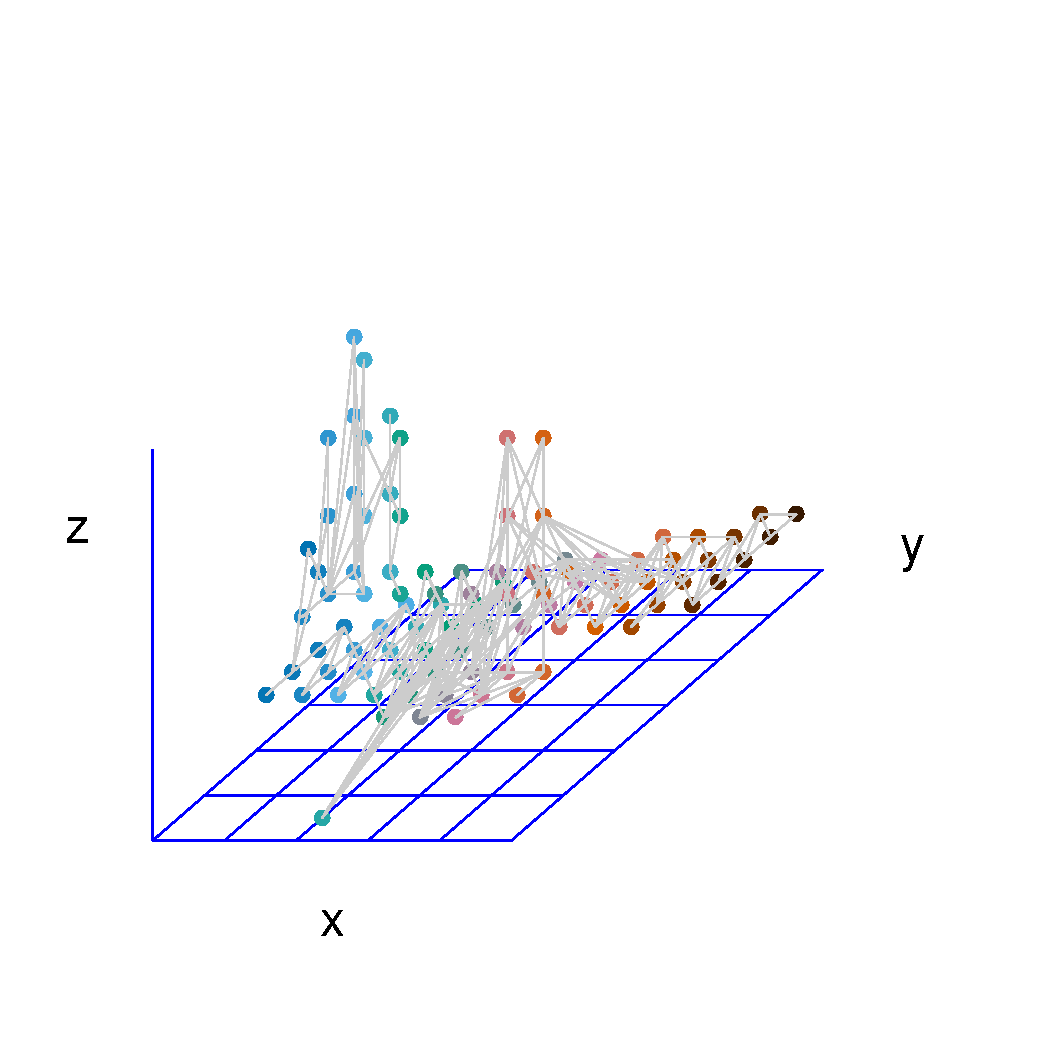
\includegraphics[width=4in]{../Figure/intro.pdf}	
	\caption{Physical location of one component of human brain network and its tracts that connect one vertex to another.}
	\label{fig:intro}
\end{figure}

Throughout this paper, assume that we are given an unweighted and undirected, connected network, equivalently graph $\boldsymbol{G}$ without self-loop, comprised of $n$ nodes for a fixed $n \in \mathbb{N}$. Even though we assume that $\boldsymbol{G}$ is undirected and unweighted, we are able to extend all of the theory here to directed and even weighted network. An adjacency matrix of a given network, denoted by $\boldsymbol{A} = \{A_{ij} : i,j= 1,..,n \}$, is often introduced to formalize the relational data of network, where $A_{ij} = 1$ if node $i$ and node $j$ are adjacent each other and zero otherwise. Let us introduce a $m$-variate ($m \in \mathbb{N}$) variable for nodal attributes $\boldsymbol{X}  \in \mathbb{R}^{m}$ which we are interested in. Investigating correlation between $\boldsymbol{G}$ and $\boldsymbol{X}$, and testing whether their distributions are independent or not is the key focus in our study. An observed network $\mathbf{G}$ can represent social network within a school and $\boldsymbol{X}$ is students' grades or heights, for example; or $\mathbf{G}$ can be a neuronal network in human brain and $\boldsymbol{X}$ is a few factors of personality. For example, Figure \ref{fig:intro} exemplifies one connected network from human brain network where dots denote nodes and tracts connected them represent edges. Location over network space, i.e. whether or how much a pair of nodes are closer than others, is different from actual spatial location, which can be measured by Euclidean distance over three-dimensional $x-y-z$ space. As correlation between spatial location of subjects and its attributes has been studied, we are going to explore correlation of subjects' attributes to their network location. 
	
The main contribution of this study is we develop multiscale test statistics which are robust to both nonlinearity and high dimensionality without modeling nor estimating networks. Having multiscale statistics is not avoidable because we regard location of or distance between nodes over network as dynamic process. We then choose the optimal scale where distance in network space and distance in attributes become most correlated each other. To explore this time-dependent distances we define a coordinate over network space at each time in the process and test independence to attributes $\mathbf{X}$. In the next methodology section \ref{sec:method}, we are going to define such multiscale distance and its properties A test statistic using multiscale distance metrics will be followed. In section \ref{sec:sim}, we demonstrate best performance of our method compared to the existing under various circumstances through numerical results. Real data example in section \ref{sec:real} show one of the applications among many.  
	
%%%%%%%%%%%%%%%%%%%%%%%%%%%%%%%%%%%%%%%%%%
	
\bigskip
\section{Methodology}
\label{sec:method}
	
First step in testing network independence to attributes is figuring out a variable which configurates location of nodes over network space. We hope that our observed network be a representative realization of this variable so that our test results can be generalized to population network. To be specific a pair of our observations for each variable we are going to test should be independent and identically-distributed(\textit{i.i.d}) realization to guarantee representativeness and avoid redundant intra-dependence.  
	
\subsection{Exchangeable Graph}
	
Assuming that we are given one network, equivalently one \textit{graph} comprised of nodes and edges. If you consider each edge as \textit{i.i.d}, then observed adjacency matrix is a random sample of a single parameter which is the probability of having edge or not. However, in this case, the resulting network model only depends on number of edges \citep{orbanz2015bayesian} and does not cover undirected or no self-loop networks, which is very common. Instead of assuming \textit{i.i.d} of edges right away, we are going to assume underlying distribution of edges and then consider a set of edges as \textit{i.i.d} conditional on random function. This idea comes from exchangeable representation of edges.
The property of exchangeability is closely related to the use of \textit{i.i.d} random variable. A graph $\mathbf{G}$ is called exchangeable if and only if its adjacency matrix $\mathbf{A}$ is jointly exchangeable \citep{orbanz2015bayesian}. 
	
	\begin{definition}[2-array exchangeability]
		\label{exchangeability}
		A random 2-array $(A_{ij})$ is called $\mathbf{\mbox{jointly exchangeable}}$ if 
		$$(A_{ij}) \stackrel{d}{=} (A_{\sigma(i) \sigma(j)})$$
		for every permutation $\sigma$ of $n$,
		and separately exchangeable if 
		$$(A_{ij}) \stackrel{d}{=} (A_{\sigma(i) \sigma^{\prime}(j) })$$
		for every pair of permutation $\sigma, \sigma^{\prime}$ of $n$.
	\end{definition}
	
However, exchangeability itself cannot guarantee being \textit{i.i.d}. Fortunately, thanks to the celebrated  \textit{de Finetti}(\ref{finetti})'s representation theorem, it has been proven that there exists a random probability measure $\eta$ on random variable $\mathbf{Z}$ that a sequence of $Z_{1}, Z_{2}, \ldots $ are \textit{i.i.d} conditional $\eta$ \textit{if and only if} the sequence is exchangeable \citep{orbanz2015bayesian, caron2014sparse}. \textit{Aldous-Hoover theorem}(\ref{Aldous_Hoover}) is the representation theorem of 2-array exchangeable array, which is useful to explain jointly exchangeable adjacent matrix. Exchangeable graph is commonly called \textit{graphon} \citep{lovasz2006limits}. Exchangeable graphon is defined through a random measurable functions \citep{chan2013estimation}.
	
\begin{definition}[graphon]
		\label{graphon}
		
		A \textit{graphon} with $n (\in \mathbb{N})$ nodes is defined as a function of a symmetric measurable function $g : [0,1]^2 \rightarrow [0,1]$ with input of $u_{i} \overset{i.i.d}{\sim} Uniform[0,1], i = 1,2,... ,n$. 
		Let $\mathbf{A}$ be an adjacency matrix of graphon. Then for any $i < j, i,j=1,2,...,n$:	
\begin{equation}
	Pr \big(   A_{ij} = 1 \big| u_{i}, u_{j} \big) = g \big(  u_{i}, u_{j} \big)
\end{equation}
\end{definition}
By \textit{Aldous-Hoover theorem}, we can now better represent exchangeable network through measurable function, but we are still halfway done in case of undirected network where $A_{ij} = A_{ji}$  $(i,j=1,2,... , n)$.  Under undirected network where self-loop is still allowed, we can represent $\{ A_{ij} : i < j \}$ as a function of $g$ of $\{ u_{i}\}$. 
	
\begin{equation}
( A_{ij} )  =  (   A_{\sigma(i) \sigma(j)}  ) \Longleftrightarrow A_{ij} \overset{ind}{\sim} Bern\big(  g(u_{i}, u_{j}) \big), i < j
\end{equation}  
	
Networks from widely used graphical model are exchangeable. One of the most popular models is Stochastic Block Model (SBM) \cite{holland1983stochastic}. 
The SBM, in the simplest setting, assumes that each of $n$ nodes in graph $\boldsymbol{G}$ belongs to one of $K \in \mathbb{N} (\leq n)$ blocks or groups. Block affiliation is important in that the probability of having edges between a pair of nodes depends on which blocks they are in.  Assume that latent variables corresponding to block affiliation follow $Z_{1}, Z_{2}, ... , Z_{n} \overset{i.i.d.}{\sim} Multinomial\big( \pi_{1}, \pi_{2}, ... , \pi_{K} \big)$. Then the upper triangular entries of $\mathbf{A}$ are independent and identically distributed conditional on $\{\mathbf{Z}\}$:
	\begin{equation} 
	A_{ij} \overset{i.i.d.}{\sim} Bern\big( \sum\limits_{k,l=1}^{K} p_{kl} I\big( Z_{i} = k, Z_{j} = l  \big)    \big), \forall  i < j.
	\end{equation}

The above distribution can also be represented through some random function $g : [0,1]^2 \rightarrow [0,1]$. Let $W_{1}, W_{2}, ... , W_{n} \overset{i.i.d.}{\sim} Unif[0,1]$ and $g\big( W_{i}, W_{j} \big) = \sum\limits_{k,l=1}^{K} p_{kl} I \big( W_{i} \in [\sum\limits_{j=0}^{k-1} \pi_{j}, \sum\limits_{j=0}^{k} \pi_{j}   ] , W_{j} \in [\sum\limits_{j=0}^{l-1} \pi_{j}, \sum\limits_{j=0}^{l} \pi_{j}  ]  \big)$, where $\pi_{0} = 0$ and $\sum\limits_{j=0}^{K}  \pi_{j} = 1$ 
\begin{equation} 
A_{ij} \overset{i.i.d.}{\sim} Bern \big( g(W_{i}, W_{j})  \big), \forall i < j
\end{equation}
Even though this is not the only representation of edge distribution, for any exchangeable graphs, including SBM and also Random dot product graph (RDPG), there exists a random function $g$ which edges are independent identically distributed conditioning on.
	
\subsubsection{Exchangeability on point process}
	
Graphon has been studied widely as a limit of random graphs \citep{lovasz2006limits}. However, despite its advantage on simple representation, it is either empty or dense. A precise definition of dense graph and sparse graph is followed by \cite{veitch2015class}. 
\begin{definition}[sparse (not dense) graph]
Let $G = \big(  V, E \big)$ be a graph and $|V|$ and $|E|$ denote the number of nodes and edges of $G$. Then graph $G$ is sparse or not dense if $|E|$ is asymptotically $o(|V|^2)$, i.e.
\begin{equation}
\frac{\sqrt{|E|}}{|V|} \xrightarrow{p} 0 \quad \mbox{as} \quad n \rightarrow \infty.
\end{equation}
\end{definition}
Thus it fails to represent real network data where sparsity or scale-free distribution is fairly common. In addition to graphon, we introduce a concept of \textit{graphex}, first proposed by \cite{veitch2015class}, which is more generalized version of graphon and also includes sparse exchangeable graphs \citep{caron2014sparse}.  \cite{caron2014sparse} suggested representing a network as a point process on $\mathbb{R}^2_{+}$ based on \textit{Kallengerg Representation Theorem} \citep{kallenberg1990exchangeable}. As we were able to represent $\{ A_{ij} \}$ through random transformation of \textit{i.i.d} uniform variables, jointly exchangeable point processing network also can be represented via a random function of \textit{i.i.d} unit rate Poisson process and uniform variables. 
To be specific, undirected graph on a point process on $\mathbb{R}^2_{+}$ can be thought of 
\begin{equation}
\mathbf{A} = \sum\limits_{i,j} A_{ij} \delta_{( \theta_{i}, \theta_{j})} 
\end{equation}	
where $A_{ij} = A_{ji} \in \{ 0 , 1  \}$ with node label space $\mathbf{\theta} \in \mathbb{R}_{+}$, $i,j = 1,2,...$, i.e. consider \texttt{Node} $i$ embedded on real line, at $\theta \in \mathbb{R}_{+}$. 	
				
\begin{definition}[graphex \cite{kallenberg1990exchangeable}]
\label{graphex}
Random graphs defined on exchangeable random measures are characterized by triple $(I, S, g)$, \textit{graphex}, where a $I \in \mathbb{R}_{+}$ is non-negative real, $S : \mathbb{R}_{+ } \rightarrow \mathbb{R}_{+}$ is an integrable function and $g : \mathbb{R}^{2}_{+} \rightarrow [0,1]$. Then conditional on $g$ and unit rate Poisson processed $\theta \times \vartheta$, random graphs $\mathbf{G}$ of graphex with node set $\{ \mathbf{\theta} \}$ is constructed as:
\begin{equation}
A_{\theta_{i} \theta_{j}} = g(\vartheta_{i}, \vartheta_{j})
\end{equation}
and exclude $\theta_{i}$ from $\mathbf{G}$ if $\theta_{i}$ is isolated and we can obtain finite subgraphs by restricting $\mathbf{\theta}  < \nu$ for some $\nu > 0$.		
\end{definition}
Then joint exchangeability applied in node itself now corresponds to joint exchangeability of a point processed node label, not on a node label itself:
\begin{definition}[Joint exchangeability on point process]
	\label{point}
	Let $h > 0$ and  $V_{i} = [h(i-1), hi ]$ for $i \in \mathbb{N}$ then
	\begin{equation}
	\big( A( V_{i} \times V_{j}  )   \big)  \stackrel{d}{=} \big( A( V_{\sigma(i)} \times V_{\sigma(j)}     \big)
	\end{equation}	
	for any permutation $\sigma$ of $\mathbb{N}$.		
\end{definition}
Complexities induced by Poisson process on node will require one more condition in testing in the next section. Despite its more intricate form, representation of sparse graph as exchangeable formation helps us to demonstrate the validity of the methods especially in real data.

%%%%%%%%%%%%%%%%%%%%%%%%%%%%%%%%%%%
\subsection{Multiscale Distance Metrics}	

\subsubsection{Diffusion maps and diffusion distance}	
There have been a lot of efforts to represent the network in terms of a summarizing network factor \citep{hoff2002latent} or some meaningful coefficients, e.g. centrality \citep{mantzaris2013dynamic, sporns2007identification}. However, there has been no node-specific variable which provides a configuration of node over network space without losing any information. \cite{coifman2006diffusion} proposed a meaningful multiscale geometries of data called \textit{diffusion maps} while keeping information on every local relation. Diffusion map is constructed via Markov chain on graph. Without any model assumption on graph, an adjacency matrix $\boldsymbol{A}$ acts as a kernel, representing a similarity between each node in $\boldsymbol{G}$; thus we do not have to estimate anything in order to obtain multidimensional representation of network topology. 
	
Let $(\boldsymbol{G}, \mathcal{A}, \mu)$ be a measure space. Throughout all of the arguments, assume that we have a countable node set with size of $n \in \mathbb{N}$. A network $\boldsymbol{G}$ is the data set of nodes and edges and $\mathcal{A}$ is a set of a pair of nodes $\{(i,j) : v_{i}, v_{j} \in V(\boldsymbol{G}) \}$. A measure of $\mu$ which represents a distribution of the nodes on $\boldsymbol{G}$, is equivalent to an adjacency matrix $\boldsymbol{A}$. A transition matrix $\mathbf{P} = \{P[i,j] : i,j=1,...,n \}$ in Markov chain of the simple random walk on $\boldsymbol{G}$, which represents the probability that flow or signal goes from Node $i$ to Node $j$, is defined as below:
	
\begin{equation}
P[i,j] = A_{ij} \big/ \sum\limits_{j=1} A_{ij}
\end{equation}
	
\begin{figure}[H]
	\centering
	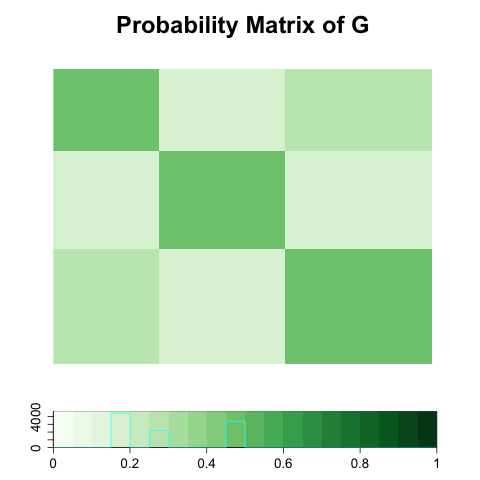
\includegraphics[width=2.3in]{../Figure/pmat.png}
	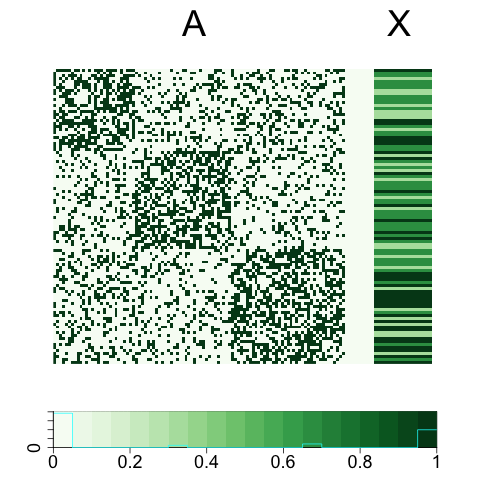
\includegraphics[width=2.3in]{../Figure/Amat.png}
	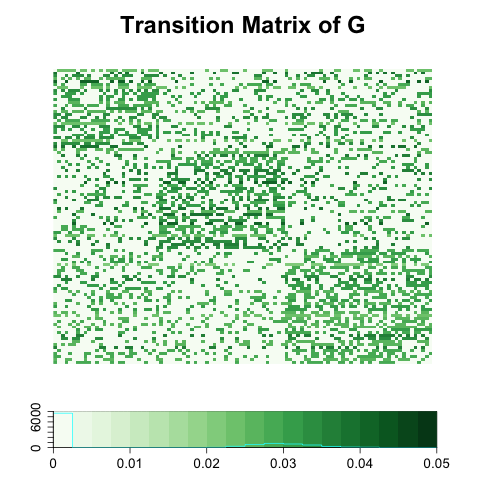
\includegraphics[width=2.3in]{../Figure/Tmat.png}
	\caption{Population probability distribution (left), realized adjacent matrix (middle), and transition matrix of sample graph $G$ from Stochastic Block Model provided in simulation (Eq. \ref{eq:Three}).}
	\label{fig:matrics}
\end{figure}	
Figure \ref{fig:matrics} illustrates one example of network $\mathbf{G}$ which follows the provided probability matrix in the left. A transition matrix $\mathbf{P}$ is a new kernel of a Markov chain of which element $P[i,j]$ represents the probability of travel from Node $i$ to Node $j$ in one time step. A corresponding probability in $t$ step is given by the $t$ th ($t \in \mathbb{N}$) power of $P$. Now we assume that diffusion process occurs within a given graph with this transition probability at each time step. Distance between a pair of nodes at each time is called \textit{diffusion distance}. That is we have distance between every pair of nodes throughout diffusion process. How to derive diffusion distance over a directed network or weighted network is provided in \cite{tang2010graph}. Other than a transition matrix, we need a stationary probability $\boldsymbol{\pi} = \{\pi(1), \pi(2), ... , \pi(n) \}$ of which $\pi(i)$ represents the probability that the diffusion process in the end is stuck in Node $i$ regardless of the starting state. In our setting, $\pi(i)$ is assumed to be proportional to the degree of Node $i$, i.e. $\pi(i) = \sum\limits_{j=1}^{n} A_{ij} \big/ \sum\limits_{i=1}^{n}\sum\limits_{j=1}^{n} A_{ij}$ ($i=1,2,..., n$).   


\begin{figure}[H]
	\centering
	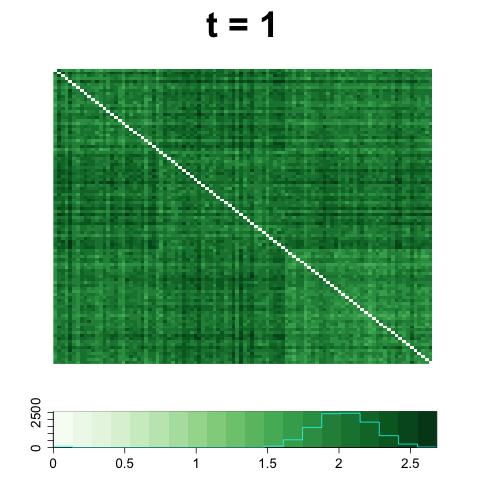
\includegraphics[width=1.5in]{../Figure/Dx1.png}
	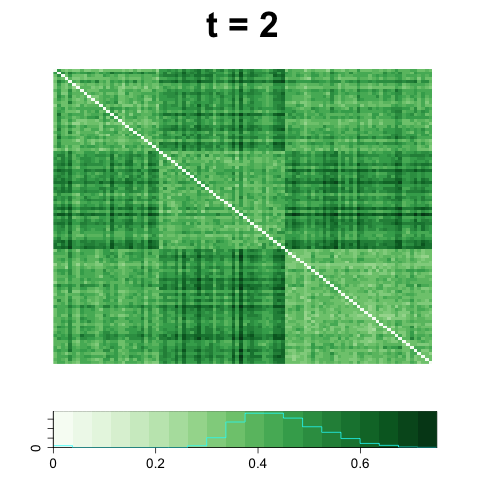
\includegraphics[width=1.5in]{../Figure/Dx2.png}
	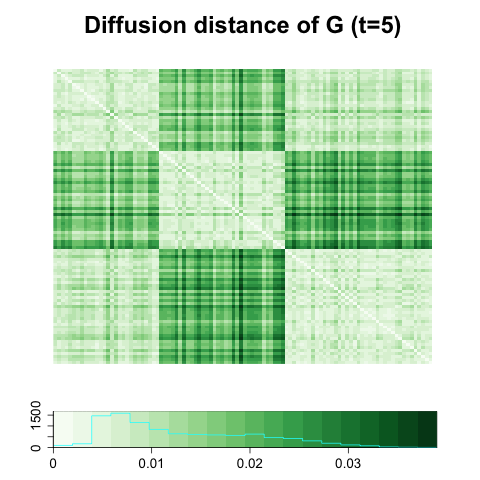
\includegraphics[width=1.5in]{../Figure/Dx5.png}
	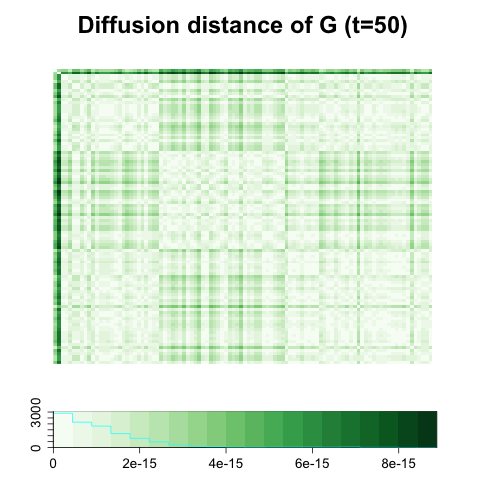
\includegraphics[width=1.5in]{../Figure/Dx50.png}
	\caption{Diffusion distance, i.e. Euclidean distance of diffusion maps at $t=1$, $t=2$, $t=5$, and $t=50$ of sample graph $G$ from Stochastic Block Model provided in simulation (Eq. \ref{eq:Three}).}
	\label{fig:diffusions}
\end{figure}	
	
For each time point $t \in \mathbb{N}$, we can define a diffusion distance $C_{t}$ defined on each pair of nodes given by :	
\begin{equation}
\label{eq:diffusion}
\begin{split}
C^2_{t}[i,j] & = \sum\limits_{w =1}^{n} \big( P^{t}[i,w] - P^{t}[j,w]  \big)^{2} \frac{1}{\pi(w)} = \sum\limits_{w=1}^{n} \left(  \frac{P^{t}[i,w]}{\sqrt{\pi(w)}} - \frac{P^{t}[j,w]}{\sqrt{\pi(w)}}   \right)^2 \\ & = \parallel P^{t}[i, \cdot] - P^{t}[j, \cdot]  \parallel^2_{L^{2}(\boldsymbol{G}, d\mu / \pi)  }
\end{split}
\end{equation}
As diffusion time $t$ increases, distance matrix $C_{t}$ is more likely to take into account distance between two nodes which are difficult to reach each other. Basically diffusion distance at fixed time $t$ measures the chance that we are likely to stay between Node i and Node j at $t$ step on our journey of all other possible paths. The higher chance is, the smaller distance between two is. Depending on the distribution of network or graph, the optimal time $t$ when the diffusion distance is most correlated to the distance in terms of $\mathbf{X}$. If you see Figure \ref{fig:diffusions}, difference between blocks in distance matrix at $t=2$ looks more distinct than that at $t=1$.  If you move to diffusion time $t=5$, you are able to distinguish every block in upper (or lower) diagonal. However if the propagation takes enough, it becomes hard to detect the differences as nodes under the peer influence are at the end assimilated. On the other hand, since it takes into account every possible path between two nodes in contrast to adjacent relation or geodesic distance, diffusion distance well reflects the connectivity. Simply speaking, connectivity between two nodes is higher if we need to eliminate more number of nodes to disconnect these two. It is more robust measure to the unexpected edges than geodesic distance. Often a set of nodes with higher connectivity have a higher propensity of having edges within this set and they are likely to form a cluster. This kind of cluster can be considered as a block in SBM. 
	
Diffusion distance of $\boldsymbol{G}$ defined as above can be represented via a spectral decomposition of its transition matrix $P$. That is, we can derive diffusion distance using its eigenvectors and eigenvalues. The spectral analysis on diffusion distance or diffusion maps have been studied mainly for its usefulness for nonlinear dimensionality reduction \citep{coifman2006diffusion,lafon2006diffusion}. 
Recall that diffusion distance at time $t$, $C_{t}$, is a functional $L^2$ distance, weighted by 1/$\pi$ in Eq.\ref{eq:diffusion}. If we transform the way to represent $C_{t}[i,j]$ slightly, we are able to obtain an orthonormal basis of $L^{2}(\mathbf{G}, d\mu / \pi)$ via eigenvalues and eigenvectors. 
Since an adjacency matrix $A$ does not guarantee a symmetric of $P$, define a symmetric kernel $Q = \Pi^{1/2} P \Pi^{-1/2}$, where $\Pi$ is a $n \times n$ diagonal matrix of which $i$th diagonal element is $\pi(i)$. Under compactness of $P$, $Q$ has a discrete set of real nonzero eigenvalues $\{ \lambda_{r} \}_{r = \{1,2,...,q \}}$ and a set of their corresponding orthonormal eigenvectors $\{ \psi_{r} \}_{r = \{1,2,..., q \} },$ i.e. $Q[i,j] = \sum\limits_{r=1}^{q} \lambda_{r} \psi_{r}(i) \psi_{r}(j)$ ($1 \leq q \leq n$).  Return to transition probability between Node $i$ and Node $j$,

\begin{equation}
\begin{split}
P[i,j] &  = \sqrt{\pi(j) / \pi(i) } Q[i,j] \\ &   = \sum\limits_{r=1}^{q} \lambda_{r} \big\{ \psi_{r}(i) / \sqrt{\pi(i)}  \big\} \big\{ \psi_{r}(j) \sqrt{\pi(j)} \big\}  \\ & : = \sum\limits_{r=1}^{q} \lambda_{r} \phi_{r}(i) \big\{ \psi_{r}(j) \sqrt{\pi(j)} \big\}
\end{split}
\end{equation}
where $\phi_{r}(i) := \psi_{r}(i) / \sqrt{\pi(i)}$. Then from $\sum\limits_{r=1}^{q} \psi^2_{r}(j) = 1$ for all $j \in \{1,2,...,n\}$, 
we can represent the diffusion distance as: 	
\begin{equation}
\begin{split}
C^2_{t}[i,j]  = \sum\limits_{r=1}^{n} \lambda^{2t}_{r} \big( \phi_{r} (i) - \phi_{r}(j)   \big)^2  
\end{split}
\end{equation}
That is,
\begin{equation}
C_{t}[i,j] = \parallel \boldsymbol{U}_{t}(i) - \boldsymbol{U}_{t}(j) \parallel
\end{equation}
where 
\begin{equation} 
\boldsymbol{U}_{t}(i) = \begin{pmatrix} \lambda^{t}_{1} \phi_{1}(i) \\ \lambda^{t}_{2} \phi_{2} (i)  \\ \vdots \\ \lambda^{t}_{q} \phi_{q}(i) \end{pmatrix} \in \mathbb{R}^{q}.
\end{equation}
Now we have  a family of $q$-variate($q \leq n$) diffusion maps $\{ U_{t} \}_{t \in \mathbb{N}} $, of which Euclidean distance is diffusion distance. Embedding each node on Euclidean metric is a novel approach in testing independence on network space; there is no estimation nor model assumption involved. However there remains a matter of dependence between observed diffusion maps.
	
\subsubsection{Properties of diffusion maps under exchangeable graphs}

We wish that diffusion maps are multivariate configuration of each node whose distance metric well reflects relative location on network space. However, due to the inter-correlated construction of $U$, e.g. $i$th subject's diffusion depends on others in the given network, it is hard to say that the observed diffusion coordinates of $n$ subjects are independent observations. As for independence of $U$, we need a concept of exchangeable graph explained in the earlier section. 

\begin{lemma}[Exchangeability and \textit{i.i.d} of $A$ in graphon]
	\label{lemma1}
Assume that a connected, undirected and unweighted graph $\mathbf{G}$ is a graphon. Then 2-array of $\{ A_{ij} : i = 1,2,... ,n , i < j \}$ are  \textit{i.i.d} conditioning on some random link function $g : [0,1]^2 \rightarrow [0,1]$. Thus for fixed row (column) of $\mathbf{A}$, $\{ A_{i1}, A_{i2}, ... , A_{in} \} \setminus \{ A_{ii} \} $ , $i \in \{ 1,2,... , n \}$ are conditionally i.i.d. on random link function $g$.  
\end{lemma}
		
From the above Lemma \ref{lemma1}, we can also prove exchangeability and conditional \textit{i.i.d} of diffusion maps at each time point. 
	
\begin{lemma}[Exchangeability and \textit{i.i.d} of $U$]
	\label{main_lemma}
	Assume that a connected, undirected and unweighted graph $\mathbf{G}$ is a graphon, i.e. any exchangeable random graph from an infinite graph. Then its transition probability $P_{ij}$ so thus  diffusion maps at fixed time $t$ also exchangeable conditional on link function of graph. Furthermore, by \textit{de Finetti's Theorem} \ref{finetti}, we can say that such diffusion maps at $t$ are conditionally \textit{i.i.d} given random probability measure $\eta$ on $U_{t}$ and random link function $g$.    
\end{lemma}
	
Lemma \ref{main_lemma} above provides us \textit{i.i.d} one-parameter family of $\{ \mathbf{U}_{t} \}_{t \in \mathbb{N}}$ conditional on a random probability measure of $\mathbf{U}_{t}$ and a random link function of $g$. At each time of $t$,  $q$-variate diffusion coordinate assigns each node to the position where $t$ step diffusion process results. Unfortunately this is a story only applied to exchangeable graph, which cannot be sparse. If we want to embed a set of nodes in sparse graphs, one more step of conditioning on point process $\mathbf{\theta}$ is needed, explained in def. $\ref{graphex}$.  
	
	
\begin{lemma}[Exchangeability and \textit{i.i.d} of $A$ in graphex]
\label{lemma2}
Assume that a connected, undirected and unweighted graph $\mathbf{G}$ is a graphex. Then 2-array of $\{ A_{ij} : i = 1,2,... ,n , i < j \}$ are  \textit{i.i.d} conditioning on some random link function $g : [0,1]^2 \rightarrow [0,1]$ and unit-Poisson process $\mathbf{\theta}$. Thus for fixed row (column) of $\mathbf{A}$, $\{ A_{i1}, A_{i2}, ... , A_{in} \} \setminus \{ A_{ii} \} $ , $i \in \{ 1,2,... , n \}$ are conditionally i.i.d. on random link function $g$ and $\mathbf{\theta}$.  
\end{lemma}	

Similar to Lemma \ref{main_lemma}, we are able to prove exchangeability of a transition matrix conditional on $g$ and also on $\theta$. Implicit interpretation of conditioning on node generating process $\theta$ is not very clear. However in testing independence between networks and nodal attributes, we are usually given a fixed number of nodes and network topology often implies edge structures. 
	
%%%%%%%%%%%%%%%%%%%%%%%%%%%%%%%%%%%%%%%%%%%%%%%%%%%%%%%%
\subsection{Applying to Multiscale Generalized Correlation}
	
\subsubsection{Distance correlation and its multiscale version}
	
Relationship between network and nodal attributes often exhibits local or nonlinear properties. Moreover, dimension of network spectrum$(q)$ often increases as a sample size increases. Unfortunately, widely used correlation measures often fail to capture nonlinear associations especially embedded in high-dimensional data set. \cite{szekely2007measuring} extended pairwise constructed generalized correlation coefficient and developed a novel statistic called distance correlation (\texttt{dCov}) as a measure for all types of dependence between two random vectors in any dimension. Let us first start from a general setting that we are given $n \in \mathbb{N}$ pairs of random samples $\{ (x_{i}, y_{i}) : x_{i} \in \mathbb{R}^{q}, y_{i} \in \mathbb{R}^{m}, i = 1,...,n \}$. Define $C_{ij} = \parallel x_{i} - x_{j} \parallel$ and $D_{ij} = \parallel y_{i} - y_{j} \parallel$ for $i,j=1,...,n$, where $\parallel \cdot \parallel$ denotes Euclidean distance defined on any vectors.   
Distance correlation (\texttt{dCor}) is defined via distance covariance (\texttt{dCov}) $\mathcal{V}^2_{n}$ of $\boldsymbol{X}$ and $\boldsymbol{Y}$, which is the following: 
	
\begin{equation}	 
\mathcal{V}^2_{n}(\boldsymbol{X}, \boldsymbol{Y}) = \frac{1}{n^2} \sum\limits_{i,j=1}^{n} \tilde{C}_{ij} \tilde{D}_{ij}
\end{equation}
, where $\tilde{C}$ and $\tilde{D}$ is a doubly-centered $C$ and $D$ respectively, by its column mean and row mean. Distance correlation $\mathcal{R}^{2}_{n}(\boldsymbol{X}, \boldsymbol{Y})$ is a standardized \texttt{dCov} scaled by $\mathcal{V}^2_{n}(\boldsymbol{X}, \boldsymbol{X})$ and $\mathcal{V}^2_{n}(\boldsymbol{Y}, \boldsymbol{Y}).$
	
\begin{equation}	 
\mathcal{R}_{n}^{2} (\boldsymbol{X}, \boldsymbol{Y}) = \frac{\mathcal{V}^2_{n} (\boldsymbol{X}, \boldsymbol{Y}) }{\sqrt{\mathcal{V}^2_{n} (\boldsymbol{X}, \boldsymbol{X}) \mathcal{V}^2_{n} (\boldsymbol{Y}, \boldsymbol{Y}) } }
\end{equation}
On the other hand, a modified distance covariance (\texttt{MCov}) $\mathcal{V}^*_{n}$ and a modified distance correlation (\texttt{MCorr}) $\mathcal{R}^{*}_{n}$ for testing high dimensional random vectors were also proposed in \cite{szekely2013distance}.   
However, \texttt{dCov} and even \texttt{MCorr} still perform not very well in existence of various nonlinear dependency and under existence of outliers (Cencheng). Out of this concern, Cencheng at al (2016) proposed Multiscale Generalized Correlation (\texttt{MGC}) by adding local scale in a sense of nearest neighbors on correlation coefficients. Multiscale version of distance covariance $\{ { {\mathcal{V}^{*}}^2_{n} }   \}_{kl}$ is defined as following : 
	
\begin{equation}
\label{eq:MGC}
{\mathcal{V}^{*}}^2_{n} (\boldsymbol{X}, \boldsymbol{Y})_{kl} = \frac{1}{n^2} \sum\limits_{i,j=1}^{n} \tilde{C}_{ij} \tilde{D}_{ij} I \big( r(C_{ij}) \leq k \big) I \big( r(D_{ij}) \leq l  \big), \quad k,l=1,2,..., n 
\end{equation}
where $r(C_{ij})$ ( $r(D_{ij})$) is a rank $\mathbf{x}_{i}$ ($\mathbf{y}_{i}$) relative to $\mathbf{x}_{j}$ ($\mathbf{y}_{j}$). It basically truncates each pairwise element of distance covariance with respect to rank in terms of (Euclidean) distance. Note that if $k=l=n$, $\mathcal{V}^2_{n}$ and ${\mathcal{V}^{*}}^2_{n}$ are equivalent. Since we call all family of $\{  {\mathcal{R}^{*}}^2_{n} \}_{k,l = 1,2,...,n}$ as \texttt{MGC} and choose the optimal set of neighborhood choice of $(k,l)$, \texttt{MGC} is more generalized version of \texttt{dCor}. How to chose the the optimal scale of $(k,l)$, $(k^{*}, l^{*})$, explained in (Cencehng) as well as its superiority and consistency. Particularly, in simulation\ref{sec:sim} we are going to show in which pattern of underlying dependency exists \texttt{MGC} is much more sensitive than global scale of statistics. 
		
\subsubsection{Choice of proper metric on network}

On the other hand, we are required a \textit{i.i.d.} node-specific coordinates of which Euclidean distance measures a distance between them in order to test independence via \texttt{MGC}. (We are not always required Euclidean metric \citep{lyons2013distance} but discussion on this is out of scope for this paper.) You might first propose directly using a column of an adjacency matrix so that we have a $n$-pair of observations $\big\{ \big( \boldsymbol{A}_{i \cdot} , \boldsymbol{X}_{i} \big) : \boldsymbol{A}_{i \cdot} = (A_{i 1} , ... , A_{i n} ), \boldsymbol{X}_{i} \in \mathbb{R}^{m}, i=1,...,n  \big\}.$ In an undirected graph, $\{ \mathbf{A_{i \cdot}}  \}$ cannot be independent. Even if it is in directed graph, Euclidean distance between $\{ \boldsymbol{A}_{i \cdot} : i =1, ... , n \}$ is not a proper metric over network space. Let us introduce a simple example. Let a given network $\boldsymbol{G}$ having 8 nodes be an unweighted, directed network and possibly allowing self-loop. Let $\boldsymbol{A}$ be its $8 \times 8$ binary adjacency matrix. Assume \texttt{Node 1}, \texttt{Node 4} and \texttt{Node 8} have the following row entries:
	
\begin{equation}
	\begin{gathered}
	\boldsymbol{A}_{1 \cdot} = \left( \begin{array}{rrrrrrrr} 1 & 1 & 1 & 1 & 1 & 1 & 1 & 1 \end{array} \right) \\
	\boldsymbol{A}_{4 \cdot} = \left( \begin{array}{rrrrrrrr} 1 & 1 & 1 & 1 & 0 & 0 & 0 & 0 \end{array} \right) \\
	\boldsymbol{A}_{8 \cdot} = \left( \begin{array}{rrrrrrrr} 1 & 0 & 0 & 0 & 0 & 0 & 0 & 0 \end{array} \right)
	\end{gathered}
\end{equation}
which results $\parallel \boldsymbol{A}_{1 \cdot} -\boldsymbol{A}_{4 \cdot} \parallel^2 = 4$,  $\parallel \boldsymbol{A}_{1 \cdot} -\boldsymbol{A}_{8 \cdot} \parallel^2 = 7$, and $\parallel \boldsymbol{A}_{4 \cdot} -\boldsymbol{A}_{8 \cdot} \parallel^2 = 3.$ Accordingly, $\parallel \boldsymbol{A}_{4 \cdot} -\boldsymbol{A}_{8 \cdot} \parallel  < \parallel \boldsymbol{A}_{1 \cdot} -\boldsymbol{A}_{4 \cdot} \parallel$. However, you can easily see that this does not make sense because \texttt{Node 4} and \texttt{Node 8} are connected each other only through \texttt{Node 1}. 
Therefore instead of using an adjacency matrix directly, we are considering embedding a vertex $v \in V(\boldsymbol{G})$ into its diffusion map of $\boldsymbol{U}$ and apply Euclidean distance metric, which is exactly same as diffusion distance. As explained before, its Euclidean distance takes into account all possible paths between every pair of nodes and measure the connectivity between them. Unlike in the other metrics in network, i.e. adjacency matrix or geodesic distance, triangle inequality holds in diffusion distance. Proof is provided in Appendix.
\begin{corollary}[Triangle inequality]
	\label{corollary1}
		For fixed time $t$, let $C_{t} : V(\mathbf{G})^2 \rightarrow \mathbb{R}_{+}$ be a diffusion distance defined on a pair of nodes in any connected and undirected graph $\mathbf{G}$. Then for any $v, w, z \in V(\mathbf{G})$,  
		\begin{equation}
		C_{t}(v,z) \leq C_{t}(v,w) + C_{t}(w,z)
\end{equation}
\end{corollary}	
	
Thanks to these properties of diffusion maps, we earn better interpretation of its Euclidean distance so that we will use it to the distance matrix in \texttt{MGC}.
	
\subsubsection{One parameter family of test statistic}

We have discussed one-parameter family \textit{i.i.d.} representation of network structures, called diffusion maps, and also discussed when given \textit{i.i.d}. pair of observations of two variables, how distance correlation and its multiscale version test independence between these two. Now it is time to combine these two.

\begin{lemma}[empirical characteristic function of conditionally \textit{i.i.d} variable]
	\label{main_lemma}
	\textcolor{red}{empirical cf of exchangeable variable converges to true cf.}
\end{lemma}	

\begin{corollary}
 \label{main.cor}
 If exchangeable random variable $\mathbf{X}^{(E)}$ and $\mathbf{Y}^{(E)}$ satisfy $E|{X^{(E)}}^2| < \infty$ and $E|{Y^{(E)}}^2| < \infty$ for each, then almost surely 
 \begin{equation}
 \lim\limits_{n \rightarrow \infty} \mathcal{V}_{n} (\mathbf{X}^{E} , \mathbf{Y}^{E} ) = \mathcal{V}(X, Y)
 \end{equation}
where $\mathcal{V}^2 (X, Y) := \| f_{X,Y}(t,s) - f_{X}(t) f_{Y}(s) \|^2$ , $X$ and $Y$ are conditionally \textit{i.i.d} random variable of $X^{(E)}$ and $Y^{(E)}$ respectively. 
\end{corollary}

Lemma \ref{main_lemma} and its following Corollary \ref{main.cor} facilitates the use of distance correlation through satisfying \textit{Theorem 2} in \cite{szekely2007measuring}.  
	
\begin{theorem}[MGC of testing independence]
 \label{theorem1}
Assume that a connected, undirected and unweighted graph $\mathbf{G}$ is an exchangeable graph, and that we are given $n$-pair of observations $\{ ( \mathbf{u}_{t}(i), \mathbf{x}_{i}): i = 1,2,... , n  , t \in \mathbb{N} \}$, where $\textbf{u}_{t}(i) \overset{i.i.d.}{\sim} f_{U_t} \big(  \eta, g \big)$, $t \in \mathbb{N}$ and $\mathbf{x}_{i} \overset{i.i.d.}{\sim} f_{X}$. Then \texttt{MGC} applied to these pair of data is theoretically consistent against all dependent alternatives in testing :
\begin{equation}
H_{0} : f_{U_t \cdot X} = f_{U_t} \cdot f_{X}.
\end{equation}
\end{theorem}
Remind that conditional distribution of $f_{U_t} \big( \eta, g \big)$ given a link function $g$ and a random probability measure $\eta_{t}$ of $\mathbf{U}_t$ has been introduced to ensure $\textit{i.i.d}$ from exchangeability. Since $\boldsymbol{U}  = \{ \boldsymbol{U}_{t} \}_{t \in \mathbb{N}}$ provides a configuration of nodes in $\boldsymbol{G},$ the above hypothesis implies testing independence between the configuration of nodes in network space and in attribute space at each time of diffusion, but as a function of a link function $g$ and a random function (variable) of $\eta$ of $\mathbf{U}$.
	
\begin{remark}
	Roughly speaking, we can say that diffusion maps are \textit{i.i.d.} function of a link function $g$ and a random function of $\mathbf{U}$ of $\eta$. Thus testing independence between conditional $U$ and $X$ can be considered as testing independence between $f \big( g, \eta \big)$ and $X$. A link function $g$ concerns the distribution of edges and a random function $\eta$ concerns nature distribution of diffusion maps. Our testing basically examines whether how edges are constructed and how diffusions(propagation) process are correlated to nodal attributes.  
\end{remark}

We are not going to state otherwise but if you assume to be given a unit-Poisson process $\{ \theta_{i} \}_{i=1}^{n}$, you can lead to the same results for sparse graphex as Theorem \ref{theorem1}. Even though we are not able to present testing results in \textit{all} alternatives, in the following section a few examples of sparse networks as well as exchangeable networks will help you understand when and why our proposing method performs better than others. 

\subsubsection{Each node's contribution to dependency measure}

In presence of nonlinear dependency or local (in)dependency, some nodes often exerts more dependence on their attributes than other nodes since the amount of dependence is not consistent over a set of nodes. Like other node-specific measure of its importance, e.g. centrality, each node's leverage on dependency measure \ref{eq:MGC} can be of interest. Here we actually measure each node's contribution to \texttt{MGC} statistic so that quantify how much its location on network space and its attributes are correlated.
Let $(k^{*}, l^{*})$ be the optimal neighborhood choice in distance matrix $(C, D)$.  Denote the contribution of node $v \in V(G)$ to the testing statistic by  $c(\cdot) : v \rightarrow \mathbb{R}$. 
\begin{equation}
\label{contribution}
c(v) = \frac{1}{2 n^2} \sum\limits_{j=1}^{n} \left\{     \tilde{C}_{v j} \tilde{D}_{v j} I \big(  r (C_{v j}) \leq k^{*}  \big) I \big( r (D_{ v j }) \leq l^{*} \big) + \tilde{C}_{j v} \tilde{D}_{j v} I \big(  r (C_{j v}) \leq k^{*}  \big) I \big( r (D_{j v}) \leq l^{*} \big) \right\} 
\end{equation}

%%%%%%%%%%%%%%%%%%%%%%%%%%%%%%%%%%%%%%%%%%%%%%%%%%%%%%%%%%%%%%%%
\section{Simulation Study}
\label{sec:sim}
	
In simulation studies presented in this paper, we make a comparison of estimated testing power across various multivariate independence test statistics: \texttt{MGC}, \texttt{dCov}, Heller-Heller-Gorfine (\texttt{HHG}) \citep{heller2012consistent}, and likelihood ratio test of Fosdick and Hoff (\texttt{FH}). For computing statistical power, we used type I error $\alpha = 0.05$ and obtain p-values of each sample network via permutations. For fair comparison between these testing methods, we also present a additive model of latent factors, which is mostly targeted by \texttt{FH}.   
	
\subsection{Stochastic Block Model}

We mentioned in the Introduction that latent network model is very common followed by the assumption of local independence. Stochastic Block Model (SBM) is one of the most popular and also useful network generative model, especially as a tool for community detection \citep{karrer2011stochastic}. We first present the simplest SBM with $K = 2$ blocks where block affiliation for each node is correlated with its attributes $X$. Let us introduce block affiliation variable $Z \in \{ 0, 1 \}$. We set If $Z_{i}  = Z_{j}$, $A_{ij} = 0.4$ and $A_{ij} = 0.1$ so that nodes in the same block are more likely to be adjacent than nodes having different value of $Z$. 
	
\begin{equation}
\small
\label{eq:twoSBM}
\begin{gathered}
	X_{i} \overset{i.i.d}{\sim} Bern(0.5), i = 1,... , n \\ 
	Z_{i}  \sim  \left\{  \begin{array}{cc} Bern(0.6) & X_{i} = 0 \\ Bern(0.4) & X_{i} = 1  \end{array} \right. \\
	A_{z_{i}, z_{j}} \sim Bern \left[  \begin{array}{cc}   0.4 & 0.1  \\ 0.1 & 0.4 \end{array}  \right]
	\end{gathered}
\end{equation}
	
Figure \ref{fig:twoSBM} illustrated two estimated power of \texttt{MGC}, \texttt{dCov}, and \texttt{HHG} based on diffusion distance and \texttt{FH}. 

\begin{figure}[H]
	\centering
	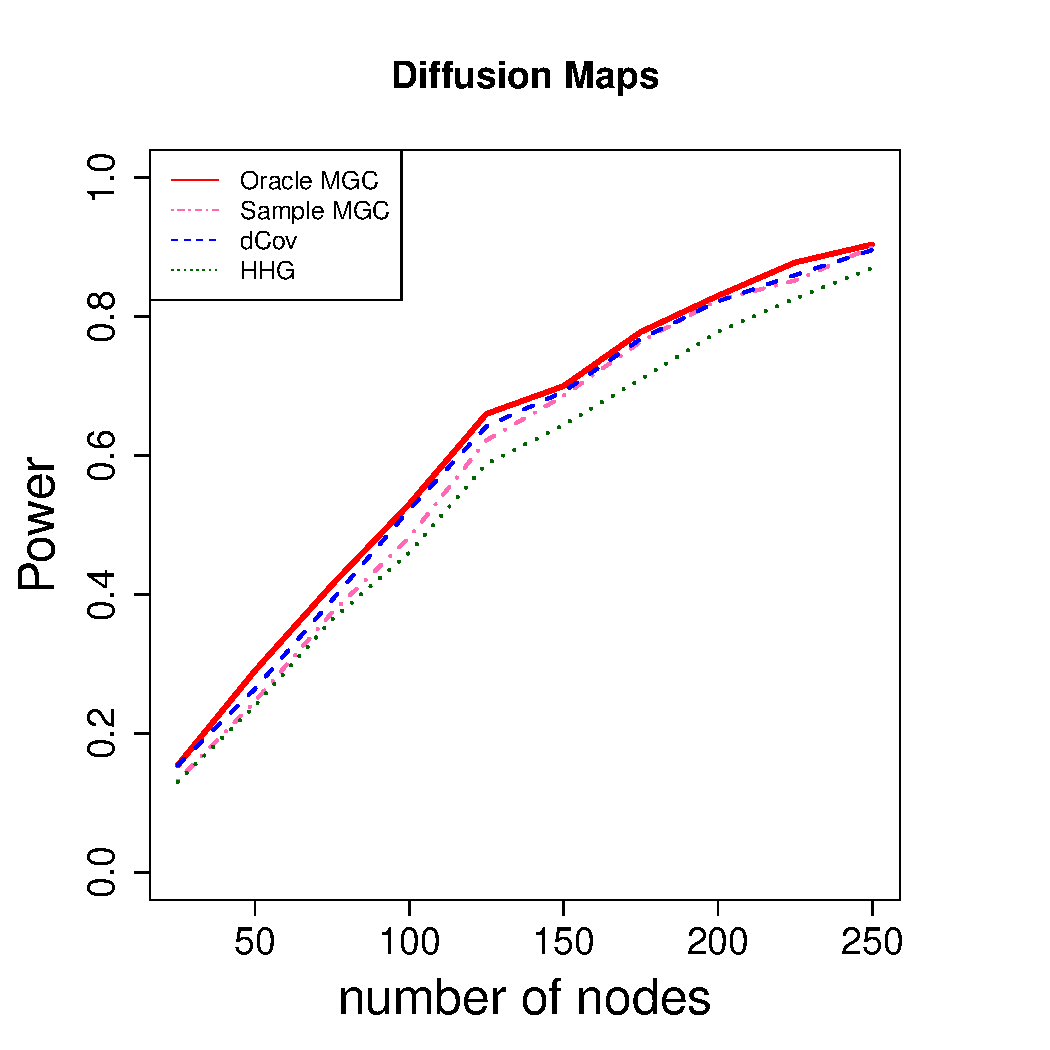
\includegraphics[width=2.3in]{../Figure/twoSBM.pdf}
	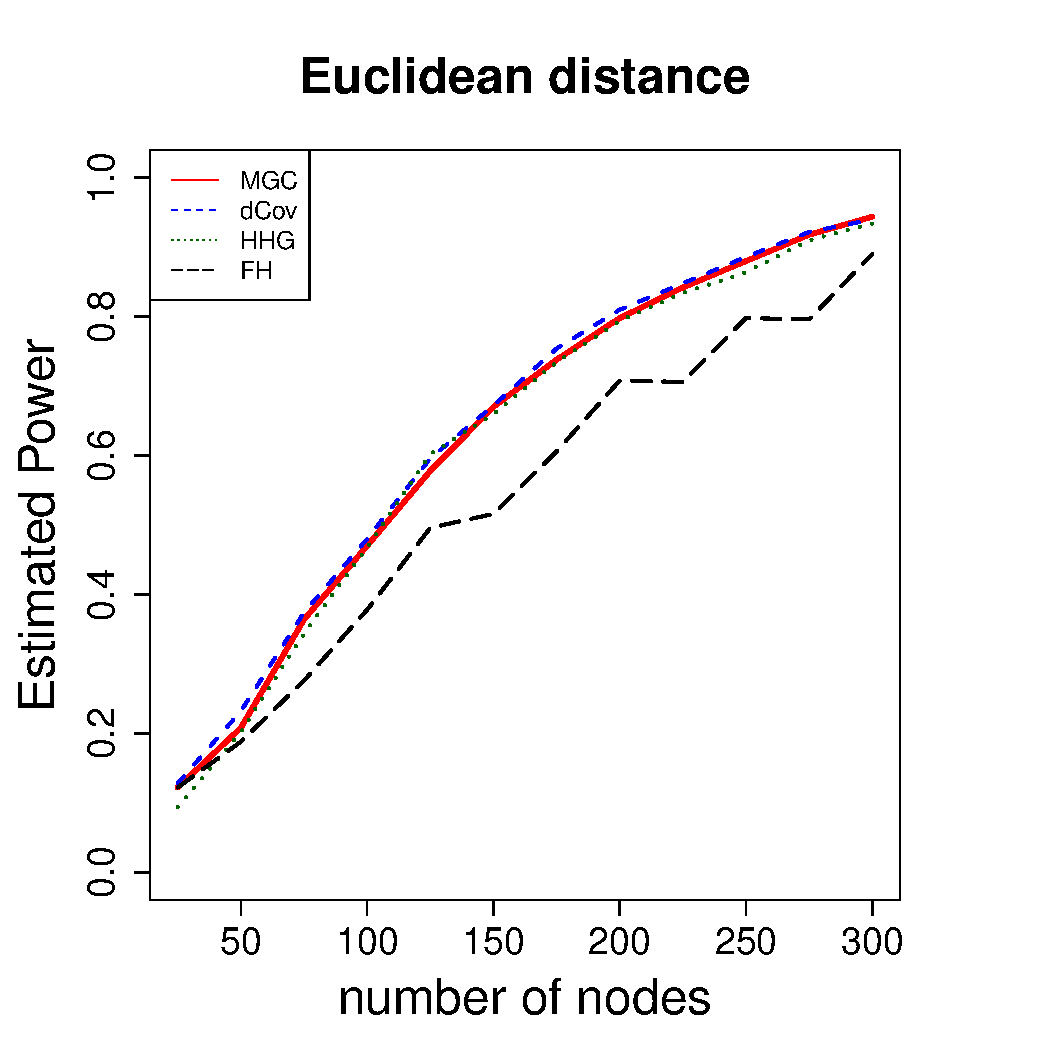
\includegraphics[width=2.3in]{../Figure/EtwoSBM.pdf}
	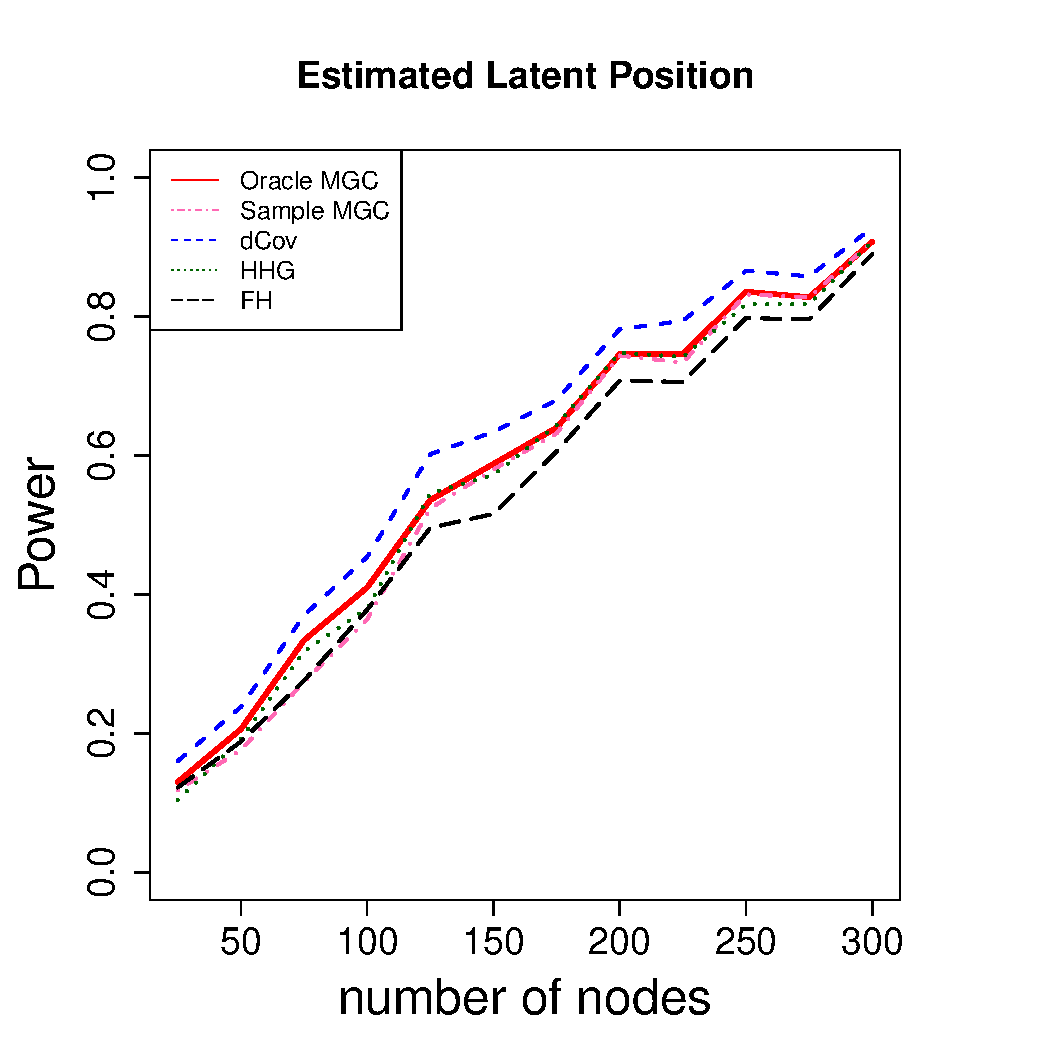
\includegraphics[width =2.3in]{../Figure/ftwoSBM.pdf}
	\caption{Estimated power based on $M = 500$ independently generated SBM presented in Eq.\ref{eq:twoSBM} using diffusion maps (left) and Euclidean of adjacency matrix (middle)  and estimated latent position(right). The most right figure contains the results of \texttt{FH} test as well.}
		\label{fig:twoSBM}
\end{figure}

\begin{figure}[H]
	\centering
	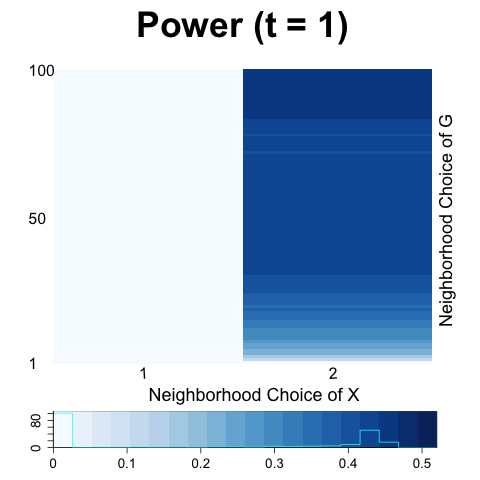
\includegraphics[width=2in]{../Figure/twoSBM_power1.png}
	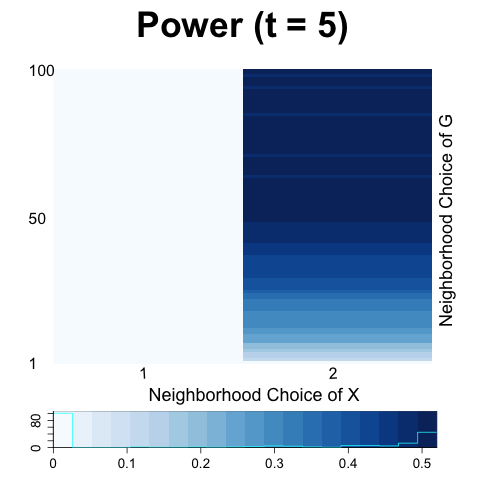
\includegraphics[width=2in]{../Figure/twoSBM_power5.png}
	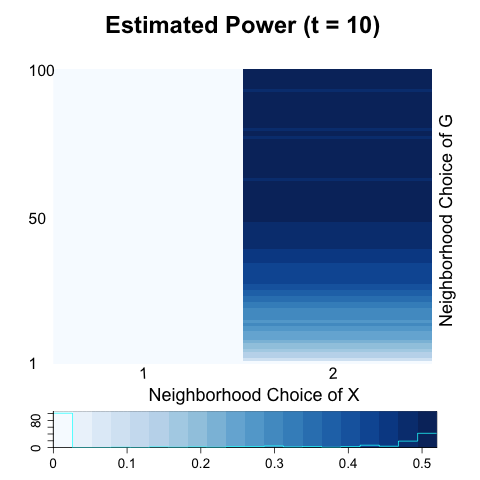
\includegraphics[width=2in]{../Figure/twoSBM_power10.png}
	\caption{Estimated power heatmap at diffusion time point $t=1$(left), $t=5$(middle), and $t=10$(right) based on $M = 500$ independently generated SBM presented in Eq.\ref{eq:twoSBM}}
	\label{fig:twoSBM_power}
\end{figure}

Higher sensitivity of \texttt{MGC} to any pattern of dependence \texttt{MGC} can be attributed both to dynamic diffusion process and optimal neighborhood choice. Figure \ref{fig:twoSBM_power} illustrates neighborhood-wise power heatmap. Note that since univariate attribute $X$ is defined binary, the heatmap looks dichotomized.

The above figures support choosing optimal neighborhood as same as global scale almost consistently across diffusion process from $t=1$ to $t=10$. This makes sense in that block affiliation exhibit global dependence on the attributes, i.e. every pair of nodes in the same block has higher probability of being adjacent. On the other hand it is still possible that nodes in different block have attribute values not monotonically dependent on the probability of having edges between them. This scheme can be realized in the following model. Let $X$ be an univariate attribute variable which has ordinal scale 1,2, and 3. 

\begin{equation}
\small
\label{eq:Three}
\begin{gathered}
X_{i} \overset{i.i.d}{\sim} Multi(1/3, 1/3, 1/3), i = 1,2, ... , n \\ 
Z_{i}  \sim  \left\{  \begin{array}{ccc} Multi(1/2, 1/4, 1/4) & X_{i} = 1 \\ Multi(1/4, 1/2, 1/4) & X_{i} = 2 \\ Multi(1/4, 1/4, 1/2) & X_{i} = 3  \end{array} \right. \\
A_{z_{i}, z_{j}} \sim Bern \left[  \begin{array}{ccc}   0.5 & 0.2 &  0.3  \\ 0.2 & 0.5 & 0. 2  \\ 0.3 & 0.2 & 0.5  \end{array}  \right]
\end{gathered}
\end{equation}

\begin{figure}[H]
	\centering
		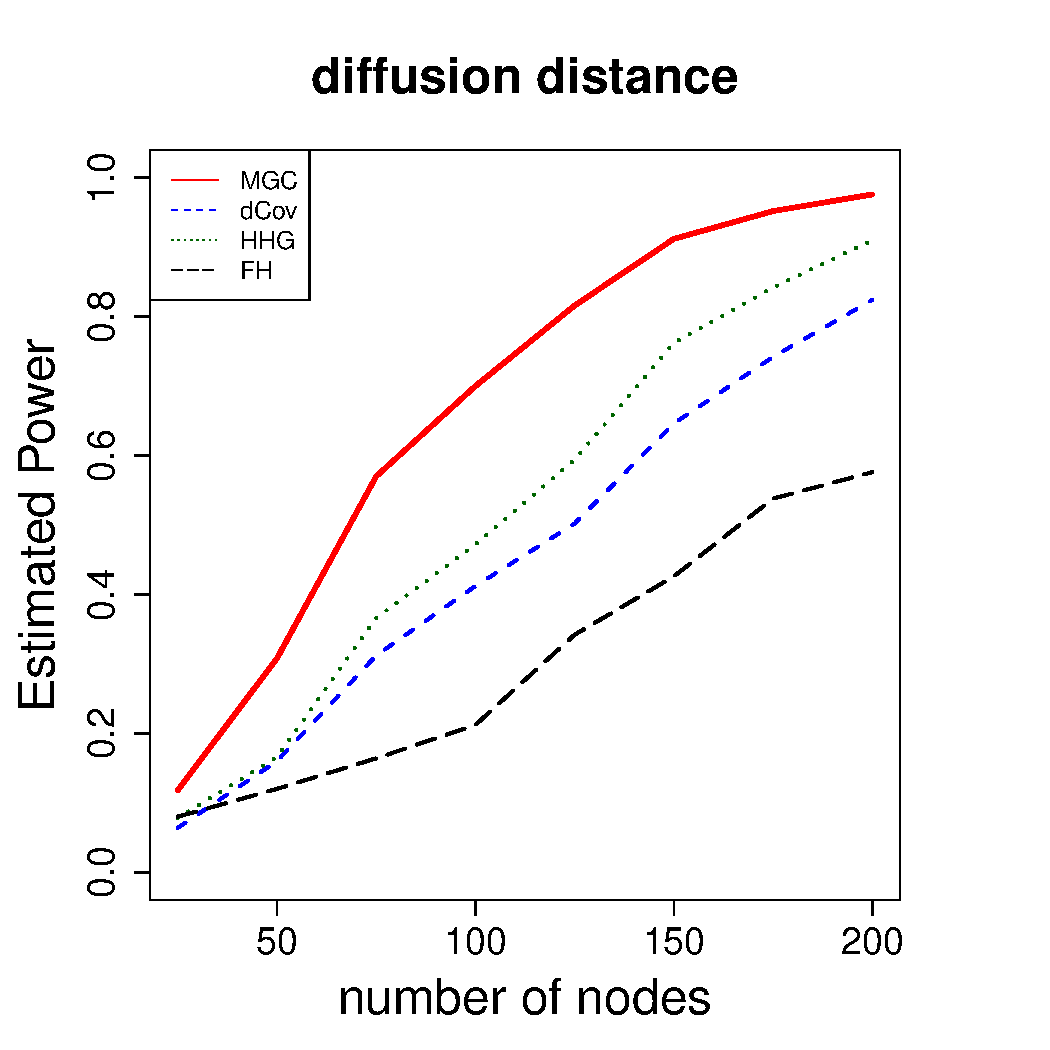
\includegraphics[width=2.3in]{../Figure/ThreeSBM.pdf}
		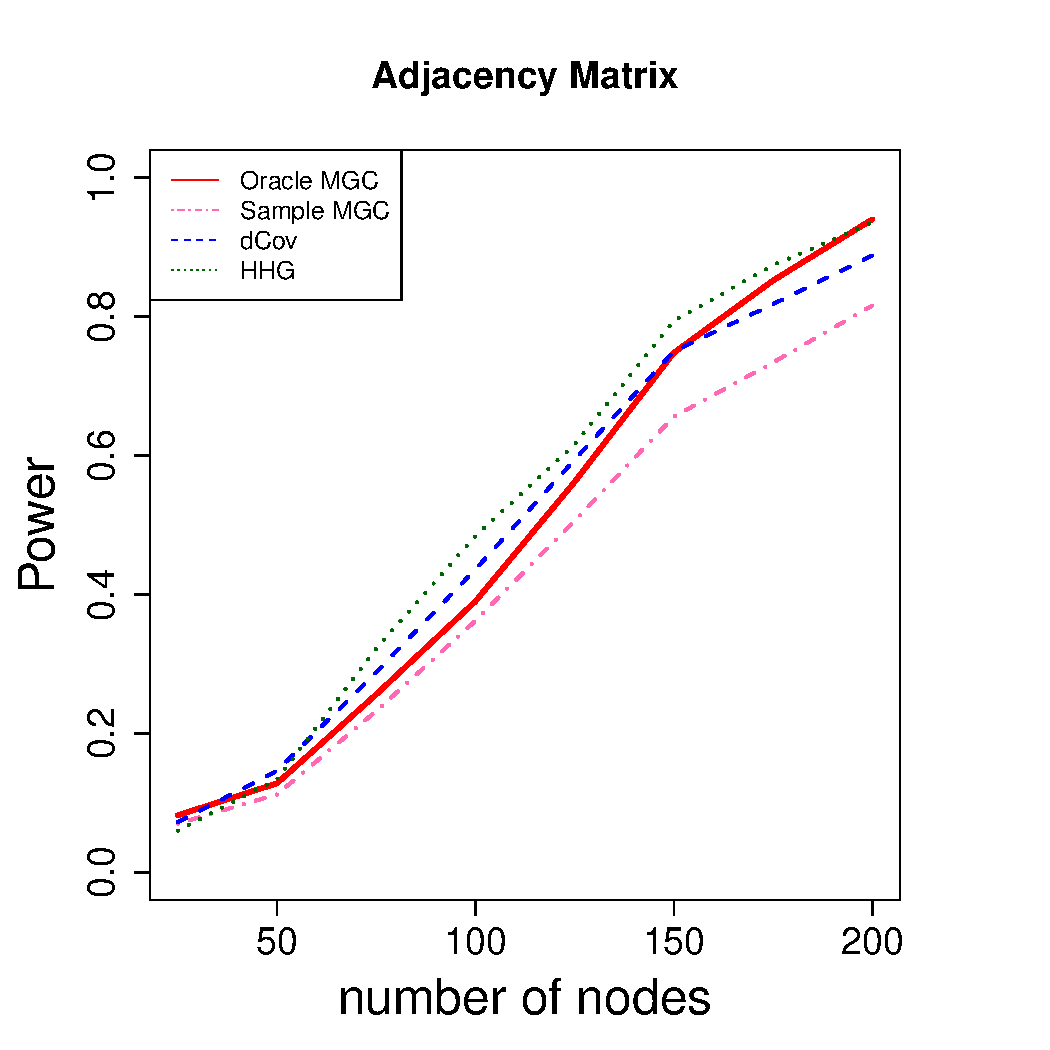
\includegraphics[width=2.3in]{../Figure/EThreeSBM.pdf}
		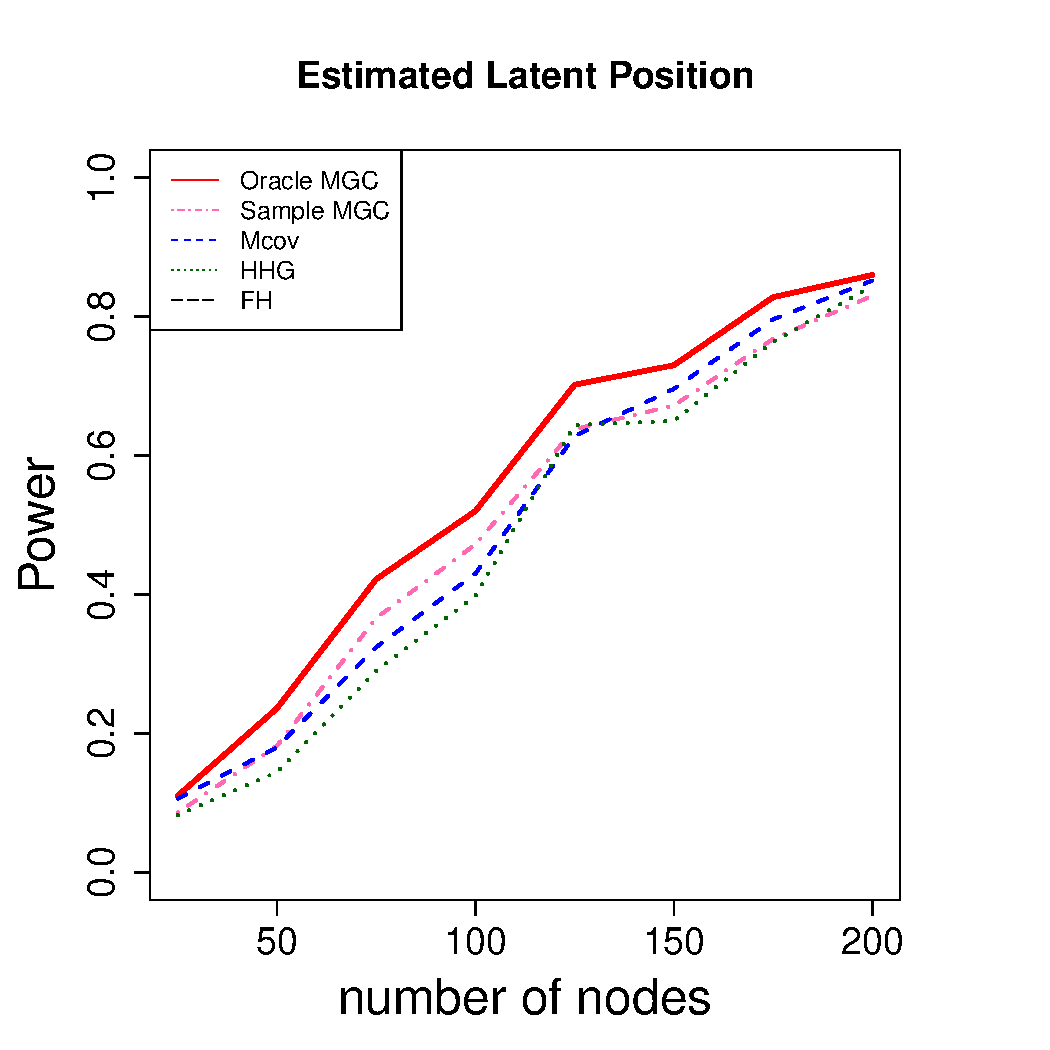
\includegraphics[width =2.3in]{../Figure/fThreeSBM.pdf}
		\caption{Estimated power based on $M = 500$ independently generated SBM presented in Eq.\ref{eq:Three} using diffusion maps (left) and Euclidean of adjacency matrix (middle)  and estimated latent position(right). The most right figure contains the results of \texttt{FH} test as well.}
			\label{fig:Three}
\end{figure}	

\begin{figure}[H]
	\centering
	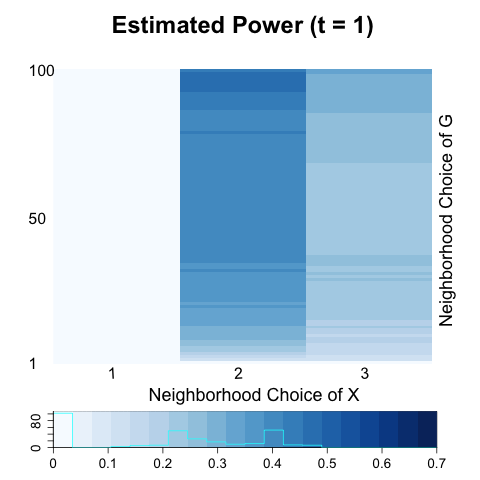
\includegraphics[width=2in]{../Figure/ThreeSBM_power1.png}
	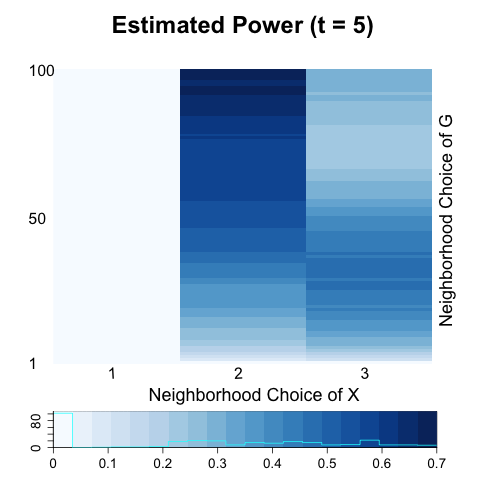
\includegraphics[width=2in]{../Figure/ThreeSBM_power5.png}
	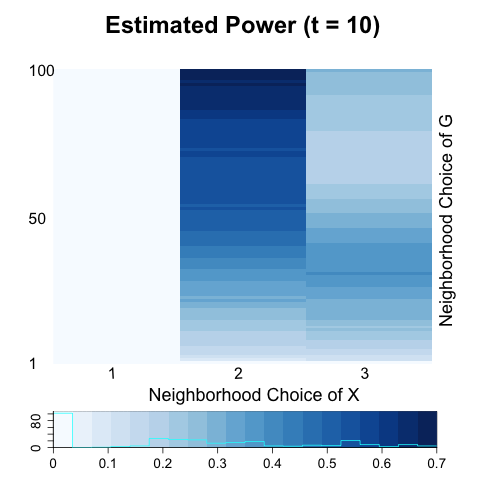
\includegraphics[width=2in]{../Figure/ThreeSBM_power10.png}
	\caption{Estimated power heatmap at diffusion time point $t=1$(left), $t=5$(middle), and $t=10$(right) based on $M = 500$ independently generated SBM presented in Eq.\ref{eq:Three}}
		\label{fig:ThreeSBM_power}
\end{figure}


Figures \ref{fig:ThreeSBM_power} demonstrates that neighborhood choice of $(k,l)$ in \texttt{MGC} statistic achieves its optimal in local scale. Roughly speaking, considering a pair of nodes in the nearest neighbor, in term of attribute values of $X$, e.g. (1,2) or (2,3), exhibits most significant dependence. If you set every pair of nodes in different blocks to have the same propensity of having edges, discrepancy between local and global scale of $(k,l)$ diminishes, which you can find in Appendix \ref{sec:appendix}.


\subsection{degree-corrected two block model}

Under SBM, we assume that all nodes within the same block have the same expected degree. However, this block model is limited by homogeneous distribution within block and provides a poor fit to networks with hubs or highly varying node degrees within blocks or communities, which are common in practice. On the other hand, the Degree-Corrected Stochastic Block model (DCSBM) proposed by \cite{karrer2011stochastic} adds an additional set of parameter, often denoted by $\theta$, to control the node degrees. This model allows variation in node degrees within a block while preserving the overall block community structure. Consider two block SBM having same distribution of $X$ and $Z$ as Eq.\ref{eq:twoSBM} but having different adjacency matrix with more variability induced by $\theta$ : 
\begin{equation}
\small
\label{eq:dcSBM}
\begin{gathered}
\theta_{i} \overset{i.i.d}{\sim} Uniform(0,2), i = 1, \ldots, n \\ 
A_{z_{i}, z_{j} | \mathbf{\theta}} \sim Bern \left[  \begin{array}{cc}  \theta_{i} \theta_{j} 0.2 &  \theta_{i} \theta_{j} 0.05  \\  \theta_{i} \theta_{j} 0.05 &  \theta_{i} \theta_{j} 0.2 \end{array}  \right]
\end{gathered}
\end{equation}

\begin{figure}[H]
	\centering
	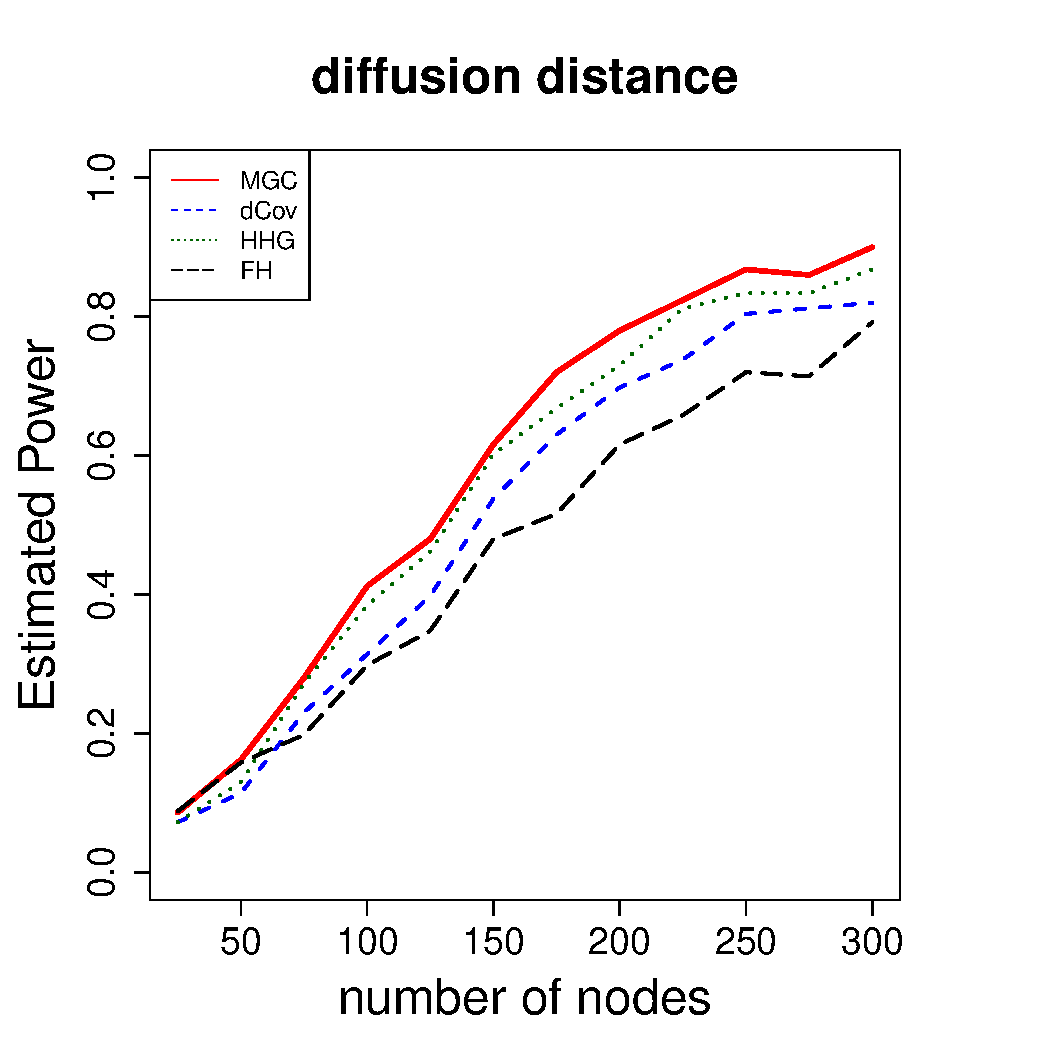
\includegraphics[width=2.3in]{../Figure/dcSBM.pdf}
	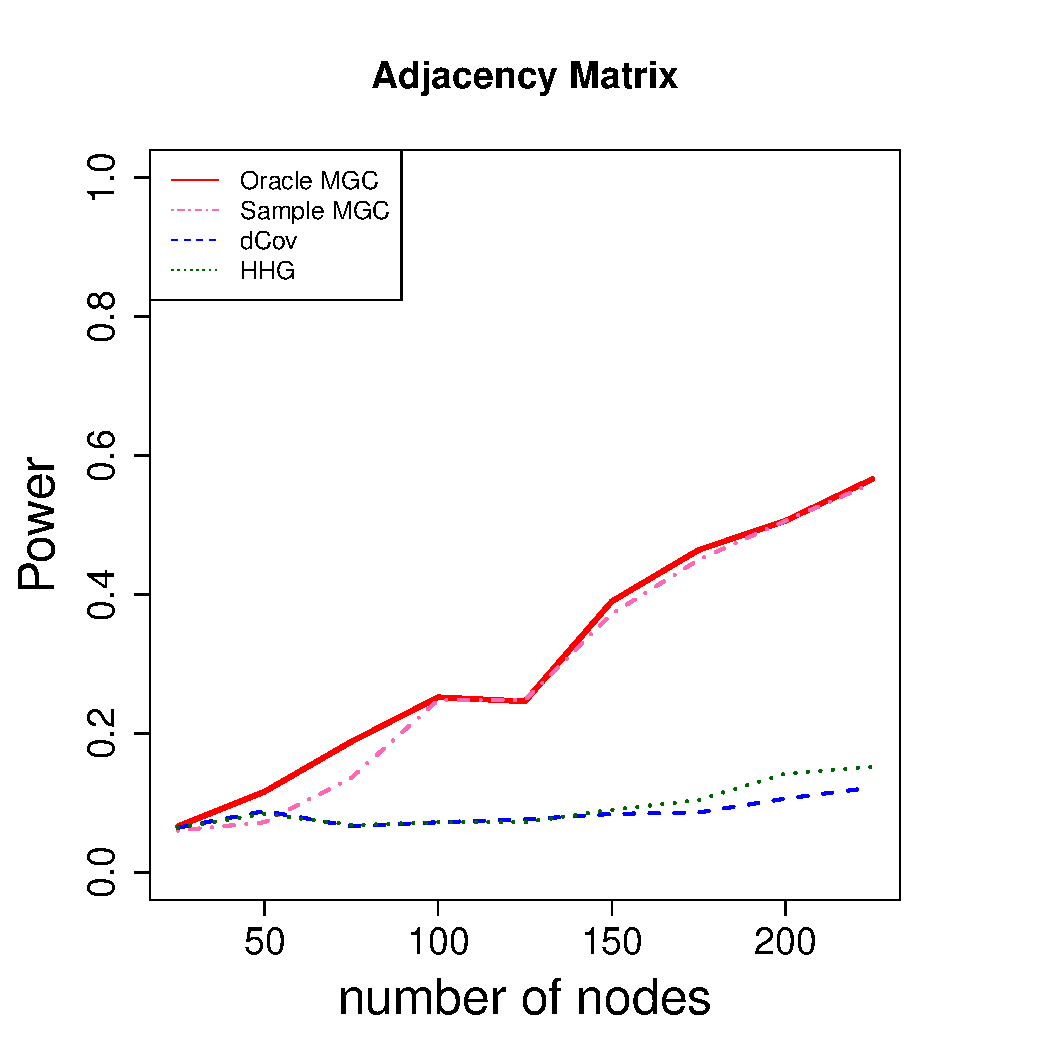
\includegraphics[width=2.3in]{../Figure/EdcSBM.pdf}
	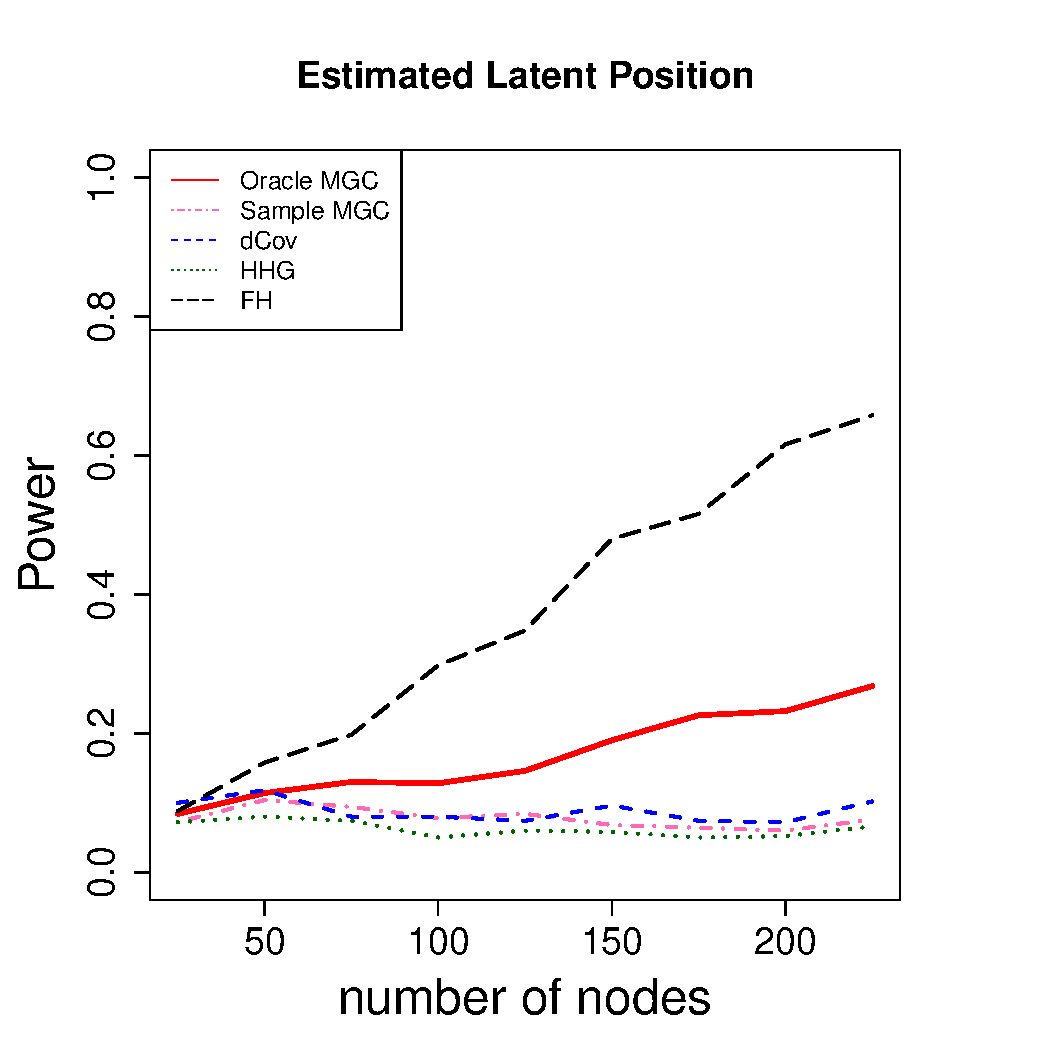
\includegraphics[width =2.3in]{../Figure/fdcSBM.pdf}
	\caption{Estimated power based on $M = 500$ independently generated SBM presented in Eq.\ref{eq:dcSBM} using diffusion maps (left) and Euclidean of adjacency matrix (middle)  and estimated latent position(right). The most right figure contains the results of \texttt{FH} test as well.}
		\label{fig:dcSBM}
\end{figure}	
	
\subsection{Additive and multiplicative graph model}

\begin{figure}[H]
	\centering
	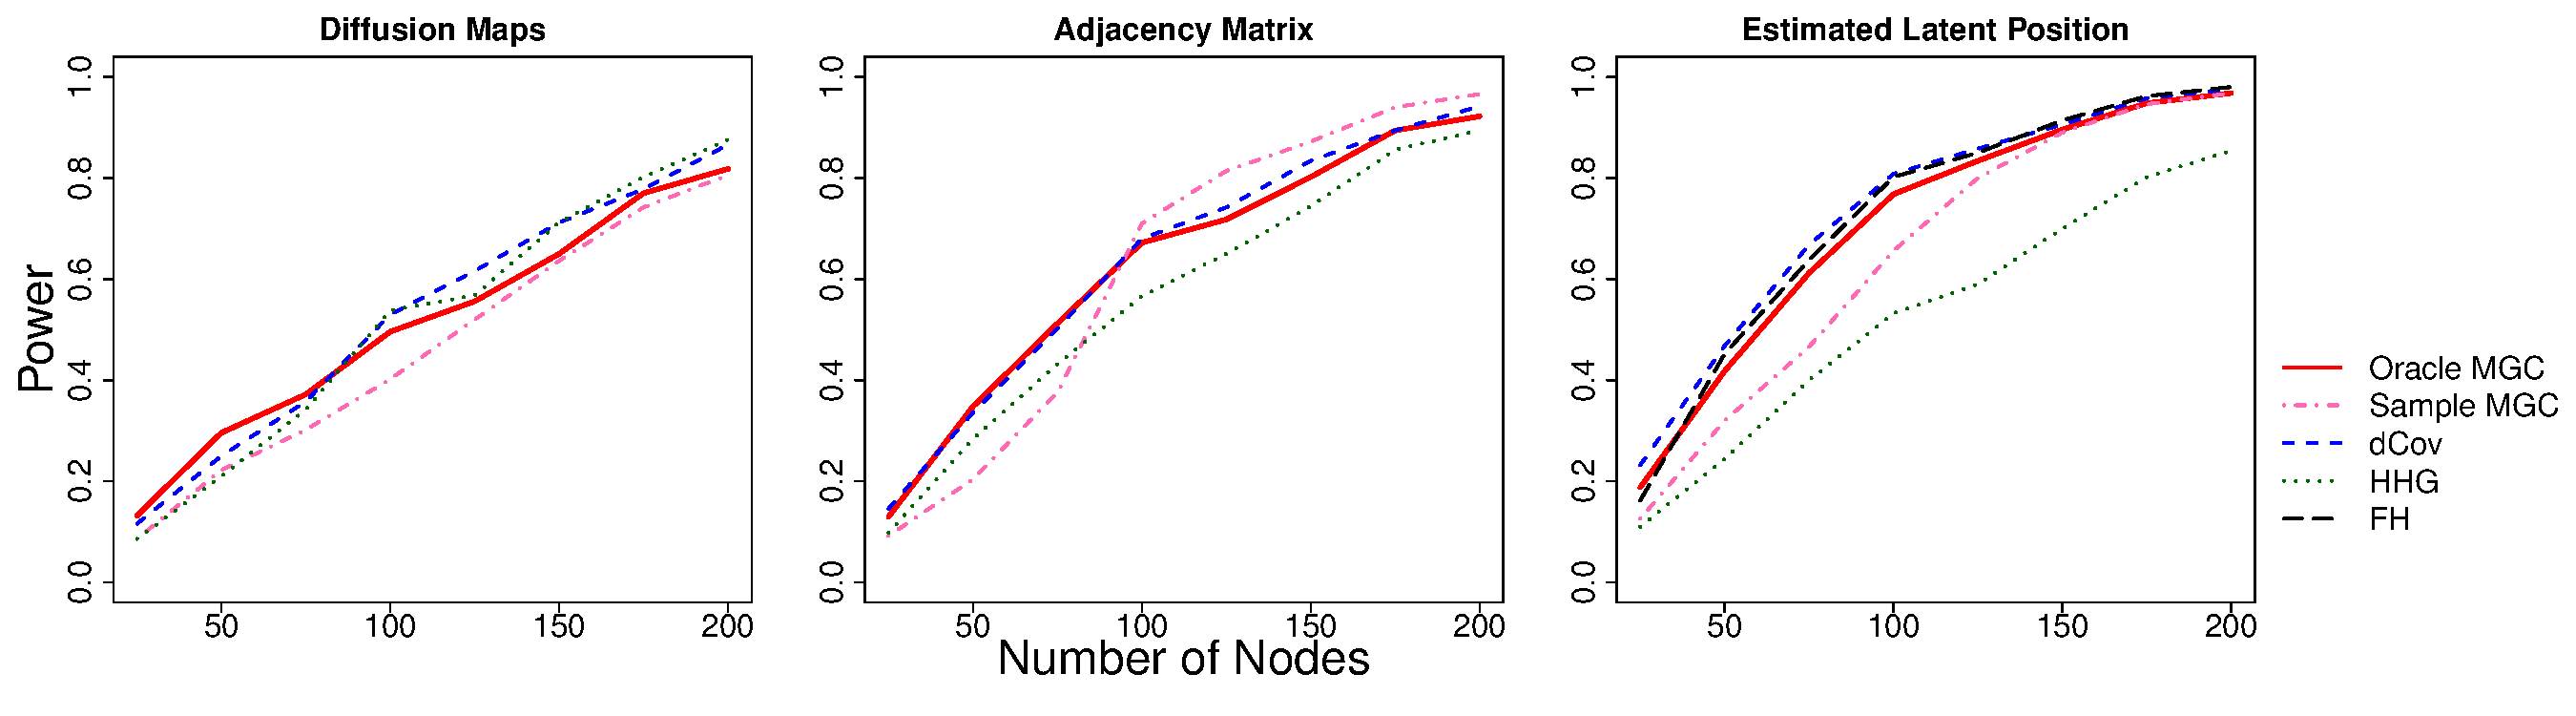
\includegraphics[width=2.3in]{../Figure/ame.pdf}
	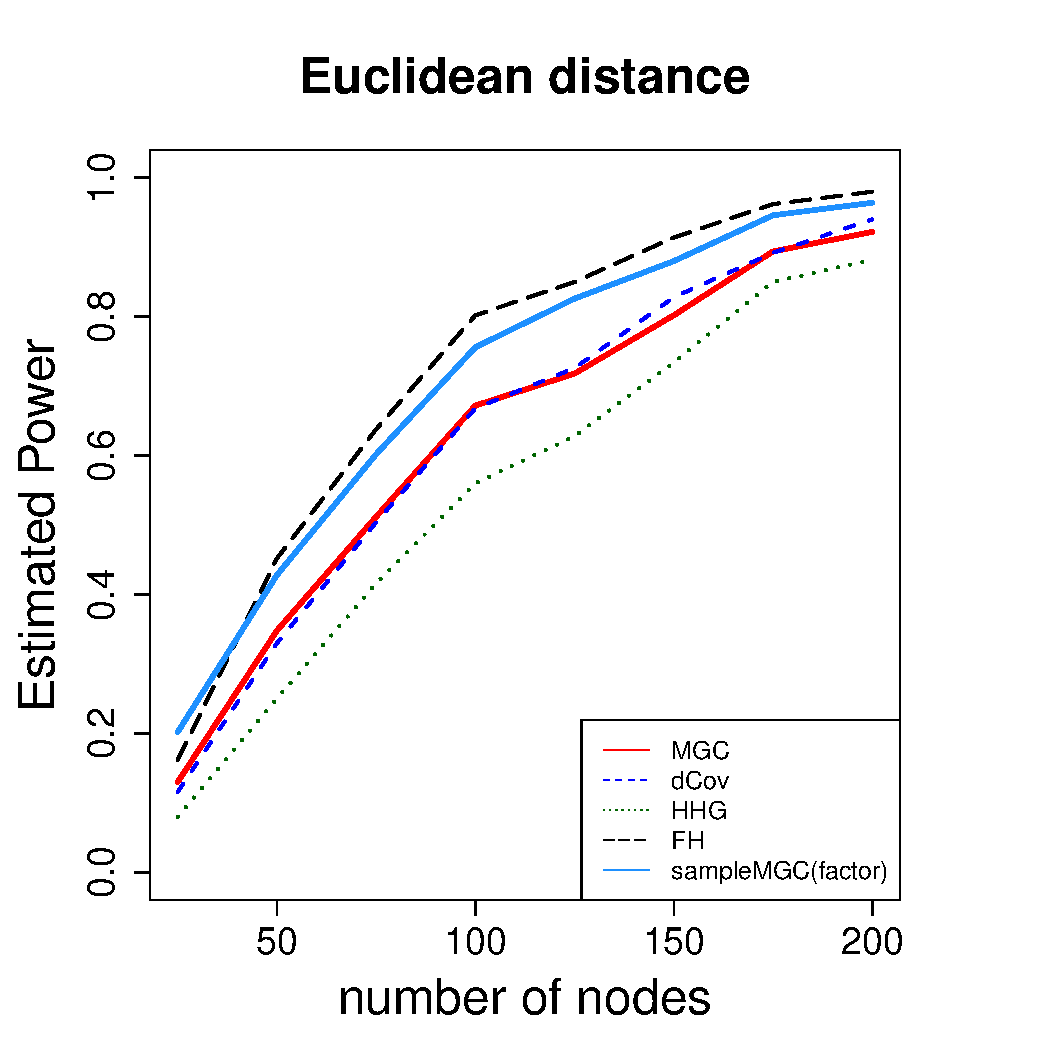
\includegraphics[width=2.3in]{../Figure/Eame.pdf}
	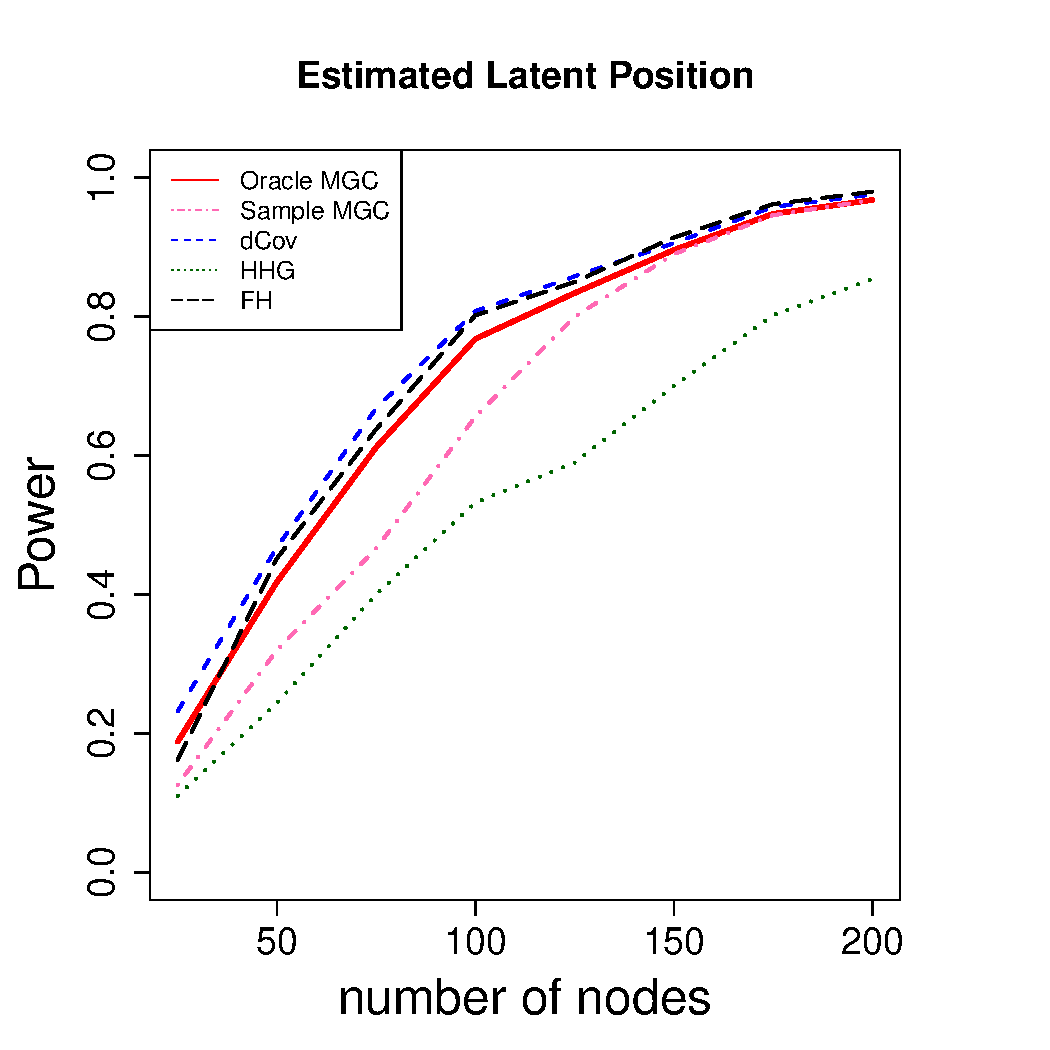
\includegraphics[width =2.3in]{../Figure/fame.pdf}
	\caption{Estimated power based on $M = 500$ independently generated SBM presented in Eq.\ref{eq:ame} using diffusion maps (left) and Euclidean of adjacency matrix (middle)  and estimated latent position(right). The most right figure contains the results of \texttt{FH} test as well.}
		\label{fig:ame}
\end{figure}

	
\cite{hoff2002latent} proposed a approach of jointly modelling network and its attributes, where networks represent additional structure via sender-specific(or row-specific) and receiver-specific(or column-specific) latent factors.
As a connection to RDPG, this model can also represented as a product of combined latent factor $\tilde{u}$ and $\tilde{v}$. 
	
\begin{equation}
\small
\label{eq:ame}
\begin{gathered}
	W_{i} \overset{i.i.d}{\sim} Uniform[0,1] \\ 
	X_{i} \overset{i.i.d}{\sim} Normal(W_{i}, 1) \\
	A_{ij}  \overset{i.i.d}{\sim} Bern \big(  ( 1 - w_{i})^2 \times (1 - w_{j})^2    \big)
\end{gathered}
\end{equation}


A family of diffusion maps are nonparametric version of embedding nodes into multivariate variable without losing any information on adjacent relationship; while \cite{fosdick2015testing} embedded nodes into network factors assuming that additive an multiplicative network model is \textit{correct}. Thus in the model explained in Eq. \ref{eq:ame}, where logit of $A$ is an additive and multiplicative function of $\{\mathbf{w} \}$, their estimated factors would be very close to the truth, much closer than embedding made from diffusion maps. However we rarely see the network which is fitted to the model in reality. If you see that your observed network actually fits to theri model, using network factors as independent observations from graph $\mathbf{G}$ and applying to \texttt{MGC} performs not very worse than \texttt{FH} statistic (Fig. \ref{fit.ame}).
Simply speaking, if network really fits well to additive and multiplicative model or we have basic knowledge about network model, we is can make sure of their node-specific additive factor $\{ a_{i} \}$ and multiplicative factor $\{ \mathbf{m}^{T}_{i} : \mathbf{m}_{i} \in \mathbb{R}^{k} \}$ in testing directly. Since they assume \textit{i.i.d} generative model for factors of each node, $\mathbf{F}_{i}$, i.e. $\mathbf{F}_{i} = \begin{pmatrix} a_{i} & \mathbf{m}^{T}_{i} \end{pmatrix} \overset{i.i.d}{\sim} MNormal$, there is nothing wrong with applying \textit{MGC} using \textit{i.i.d} observations of $\{ \mathbf{F}_{i}, \mathbf{X}_{i} \}$.   
	


\subsection{Exchangeable graph on Poisson process}

We have discussed SBM and its derivative dcSBM in consideration of real network data. However an exchangeable network defined as Def. \ref{exchangeability} is still dense. Here we revisit the example of graphex which is provided in \cite{veitch2015class}, which has power-law degree distribution.
\begin{equation}
\small
\begin{gathered}
N_{\nu} \sim Poi( c \nu) \\ 
\{ \theta_{i} \} \big| N_{\nu} \overset{iid}{\sim} Uniform[0, \nu]  \\ 
\{ \vartheta_{i} \} \big| N_{\nu} \overset{iid}{\sim} Uniform[0,1] \\ 
\{ X_{i}  \} | N_{\nu} \overset{ind}{\sim} Normal \big( \vartheta_{i}, 10 \big)  \\ 
(\theta_{i}, \theta_{j}) \big| W, \vartheta_{i}, \vartheta_{j} \overset{ind}{\sim} Bernoulli \big( W\big( \vartheta_{i}, \vartheta_{j} \big) \big) 
\end{gathered}
\end{equation}
where $W(\vartheta_{i}, \vartheta_{j} ) = (\vartheta_{i} + 1)^{-2} ( \vartheta_{j} + 1 )^{-2}$ or 0 if $\vartheta_{i} = \vartheta_{j}$. 



%%%%%%%%%%%%%%%%%%%%%%%%%%%%%%%%%%%%%%%%%%%%%%%%%%%%%%%%%%%%%%%%
\section{Real Data Examples}
\label{sec:real}
	
\subsection{MRI}
	
\textcolor{red}{needs contexts}	
	
We look into one of the connected components with $n = 95$ nodes of whole disconnected network. 
	
$\{ \mathbf{U}_{t} \in \mathbb{R}^{95} \}_{t \in \mathbb{N}}$ $\mathbf{X} = (x,y,z) \in \mathbb{R}^{3}$
	
It turns out that $q=95$, i.e. full rank of transition matrix. In other words we are testing independence between 95-dimensional diffusion maps and 3-dimensional nodal attributes at each $t \in \mathbb{N}$.
	
	
test independence between brain network and its 3-dimensional locations; test independence between functional location and physical location. 
	
\begin{figure}[H]
	\centering
		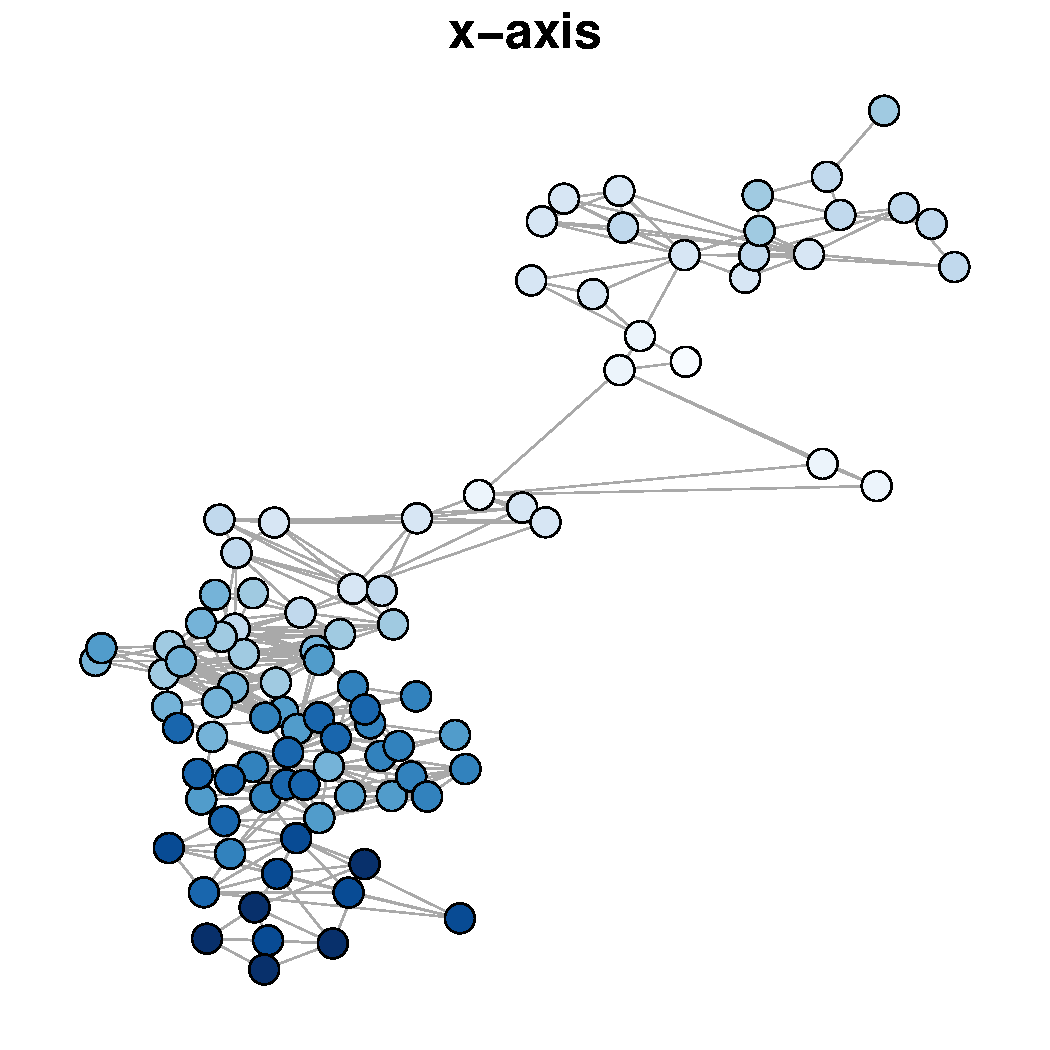
\includegraphics[width=1.5in]{../Figure/brain1_x.pdf}
		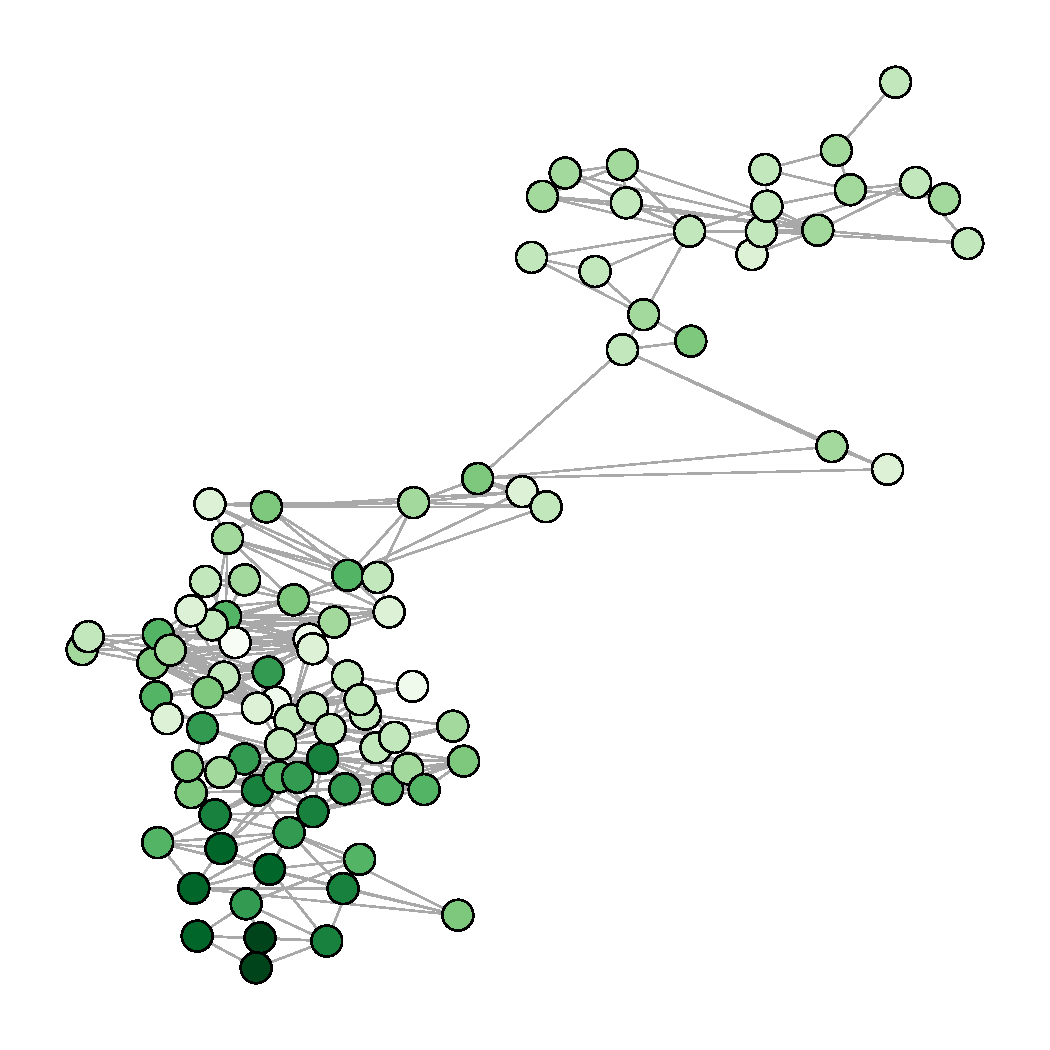
\includegraphics[width=1.5in]{../Figure/brain1_y.pdf}
		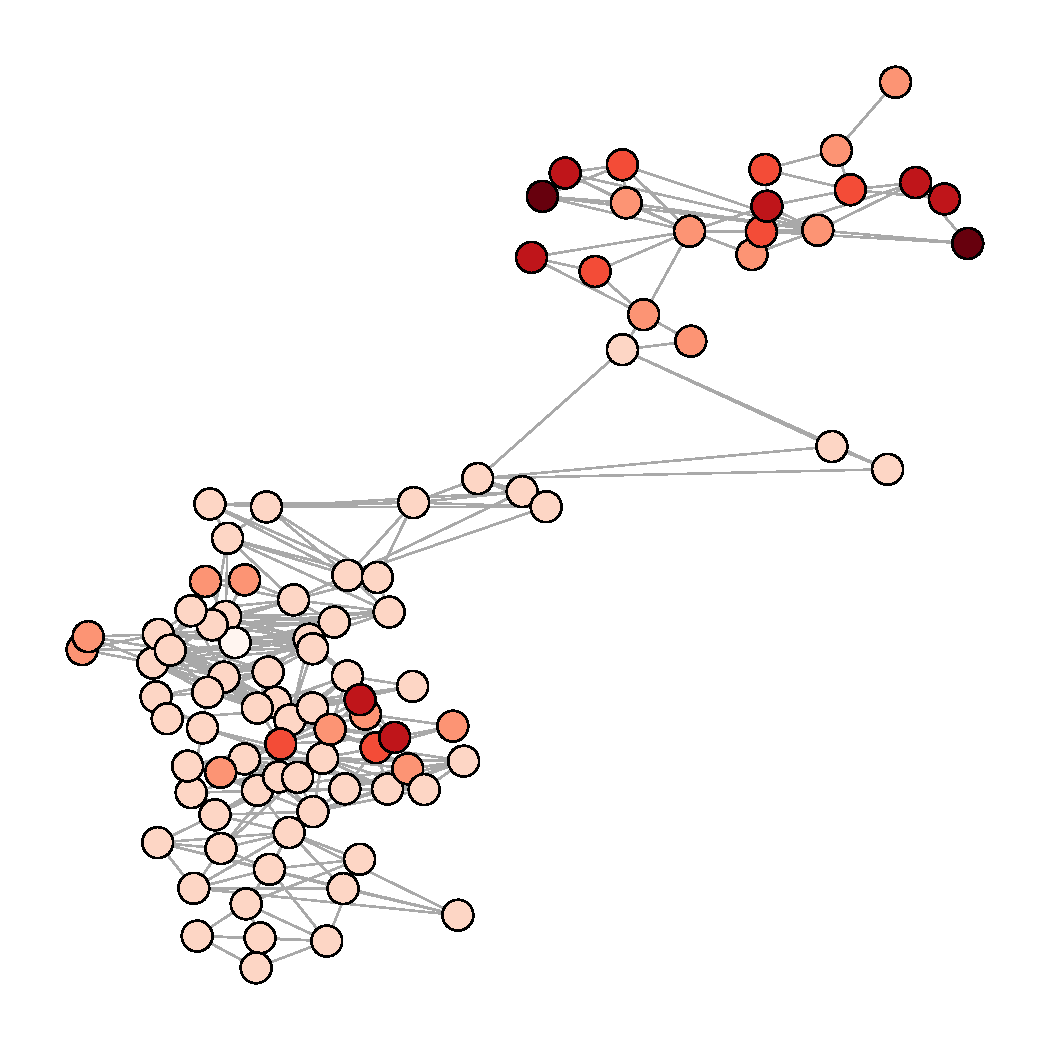
\includegraphics[width=1.5in]{../Figure/brain1_z.pdf}
		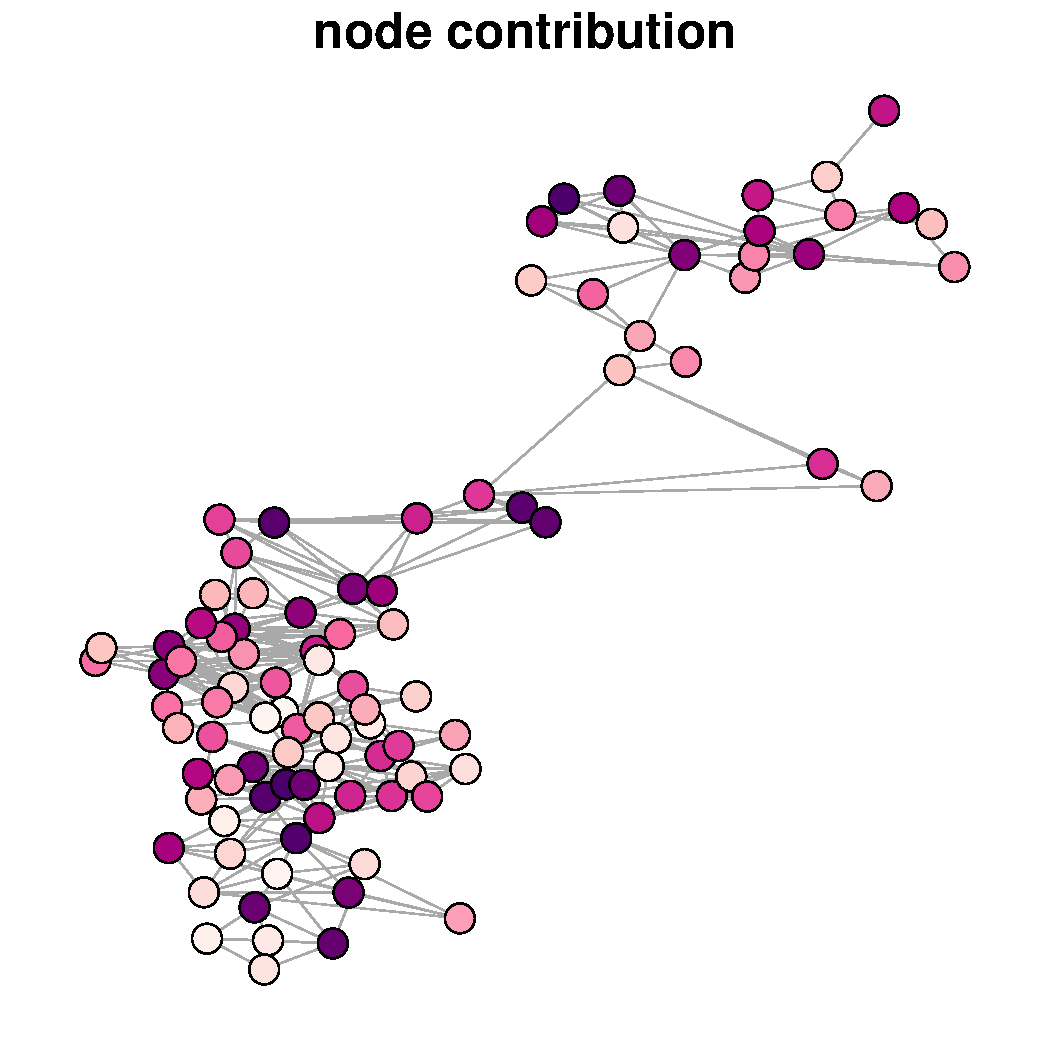
\includegraphics[width=1.5in]{../Figure/brain1_weight.pdf}
	\caption{Subnetwork of MRI network. Darker colored nodes indicate higher positioned node in terms of $x$-axis(left), $y$-axis(middle), and $z$-axis(right).}
		\label{fig:mri}
\end{figure}
	
	
\section{(one more example that MGC or diffusion  works differently )}	
	
%%%%%%%%%%%%%%%%%%%%%%%%%%%%%%%%%%%%%%%%%%%%%%%%%%%%%%%%%%%%%%%%
\section{Discussions}
\label{sec:discussion}
	
Throughout this study, we demonstrate that multiscale network test statistic to test network independence between network and its nodal attributes performs well in diverse settings, being supported by thorough theory on distance correlation and diffusion maps. These two tools are both specialized in detecting local and nonlinear dependence patterns, which other existing methods are lack of. However testing independence is often the very first step in investigating relationship between network topology and nodal attributes in our interest. It is more likely that we want to know more than binary decision of rejecting or not rejecting the hypothesis. Multiscale test statistics attributed to both neighborhood choice $\{ (k,l)  \}$ and time spent in diffusion processes $\{ t \}$ provides us a hint on latent dependence structure as well.  However due to the ambiguousness of saying \textit{optimal}, our work has some limitations; we do not suggest any theoretically supported tools to select the \textit{optimal} time to obtain p-values of test statistics. We may further want a family of p-values as a function of $t$. Future research can be focused on restoring true dependence pattern or estimating \textit{optimal} scale from a family of statistics. On the other hand, obtaining a full family of statistics are also computationally infeasible; at every Markov process, we chose the optimal region of neighborhood. As an ad hoc, we selected optimal $t$ with highest power or lowest p-values from 1 to 10 for our simulation \ref{sec:sim}.  Other than these computational issues, someone might be uncomfortable about being conditioned by a random function of $g$ and $\eta$.  However, we have to say that this is inevitable in order to argue sample properties of being \textit{i.i.d.}, which is also very conceptual and impossible to prove. Through conditioning diffusion maps $\{ \mathbf{U}_{t} \}$ by unknown network generative model $g(\cdot, \cdot)$ and also unknown diffusion process model $\eta(\cdot)$, we are finally able to assert that our observations are a fair sample eligible for test. 
	
Despite a few shortcomings listed above, a range of applications of \texttt{MNT} statistics and node-specific representation of network is very diverse. Especially multiscale version of test would be very useful when indirect networking through diffusion process is not ignorable or cluster membership significantly affects attributes. Furthermore even though we specifically constraint the statistic into testing independence between network and nodal attributes, we are able to implement independence testing of two networks with same size by inputting diffusion distance at each time point from each of network in Eq. \ref{eq:MGC}. This type of test will be useful when we want to show a pair of networks are topologically or structurally independent. For example, we might wonder if network on \textit{Facebook} and network induced by club activity within class or school are independent or not; if DNA methylation network is correlated with gene expression network \citep{bartlett2014dna} so that the behavior of interest measured by DNA methylation network can be matched to that noticed by gene expression network, etc.  In a broad sense, we suggest the proper metric applied to network and justify its use in measuring correlations between \textit{network vs. attributes} or \textit{network vs. network}. Even though we have fully presented procedures, e.g. testing on diffusion maps from $t=1$ to $t=10$  and obtaining a family of all local scales for each, depending on the previous knowledge or on the results of model fitting, you may shorten the steps as well. We also presented the case where additive and multiplicative models work pretty well and how to modify the statistic in this case. Likewise the application and variation of multiscale network test is almost limitless. 


 	
%%%%%%%%%%%%%%%%%%%%%%%%%%%%%%%%%%%%%%%%%%%%%%%%%%%%%%%%
\appendix
\section{appendix}
\label{sec:appendix}
\subsection{supplementary figures}

\begin{equation}
\small
\begin{gathered}
	X_{i} \overset{i.i.d}{\sim} Multi(1/3, 1/3, 1/3), i = 1,2, ... , n \\ 
	Z_{i}  \sim  \left\{  \begin{array}{ccc} Multi(1/2, 1/4, 1/4) & X_{i} = 1 \\ Multi(1/4, 1/2, 1/4) & X_{i} = 2 \\ Multi(1/4, 1/4, 1/2) & X_{i} = 3  \end{array} \right. \\
	A_{z_{i}, z_{j}} \sim Bern \left[  \begin{array}{ccc}   0.5 & 0.2 &  0.2  \\ 0.2 & 0.5 & 0. 2  \\ 0.2 & 0.2 & 0.2  \end{array}  \right]
\end{gathered}
\end{equation}

\begin{figure}[H]
	\centering
	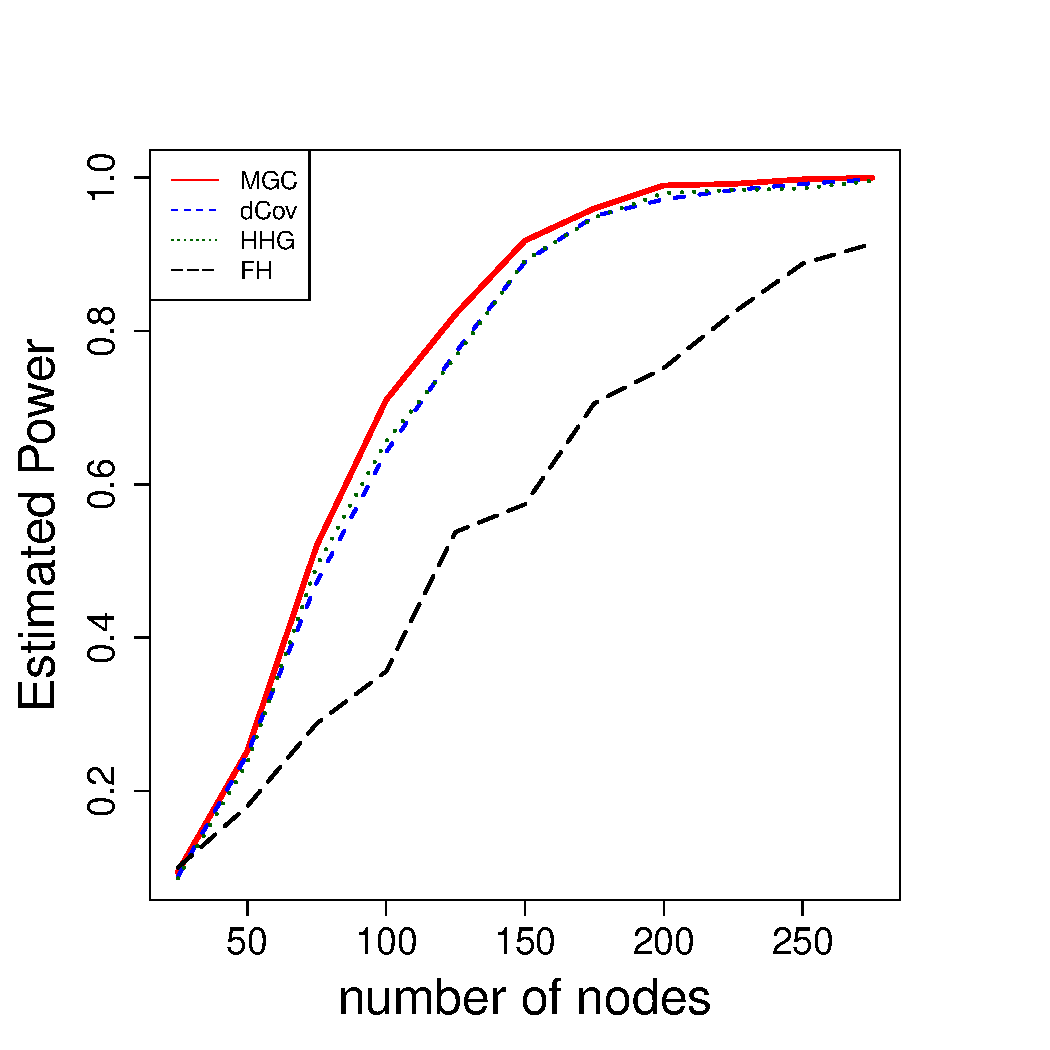
\includegraphics[width=3in]{../Figure/threeSBM_2.pdf}
	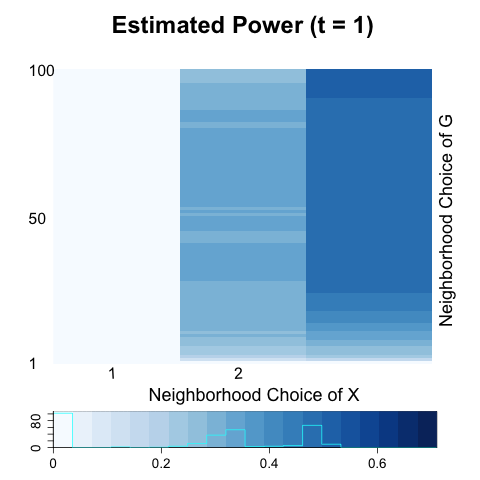
\includegraphics[width=2in]{../Figure/threeSBM_power1_2.png}
	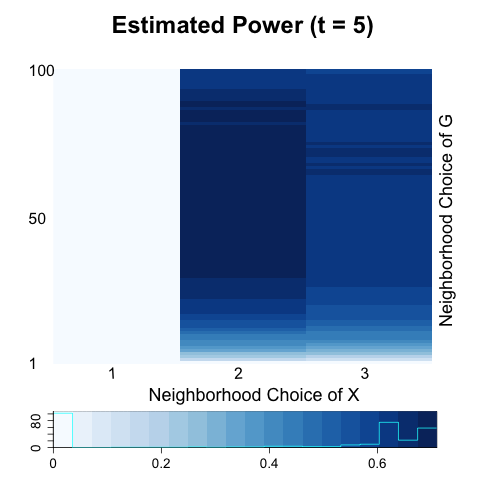
\includegraphics[width=2in]{../Figure/threeSBM_power5_2.png}
	\caption{Estimated optimal power based on diffusion maps and \texttt{FH} test statistics (left) and estimated power heatmap using \texttt{MGC} when sample size $n = 100$ (right).}
		\label{fig:threeSBM}
\end{figure}
%%%%%%%%%%%%%%%%%%%%%%%%%%%%%%%%%%%%%%%%%%%%%
\newpage
\subsection{Algorithms}
\alglanguage{pseudocode}

\begin{algorithm}[H]
	\caption{Mutiscale representation of nodes in network}
	\begin{algorithmic}[1]
		\Require Transition probability matrix of network $G$ and time points($\in N$) of diffusion time. 
		\Ensure A list of diffusion maps at each time point.
		\Function{ \texttt{dmap} }{ $n \times n$ transition matrix $P$, time points $\{ t_{1}, t_{2}, \ldots, t_{K} \}$ } 
		\State $\mathbf{\pi} :=$ \texttt{statdistr}($P$)\Comment{stationary distribution of $P$} 
		\State $\Pi : =$ \texttt{Diag}($\mathbf{\pi}$)\Comment{Diagonal matrix with diagonal element of $\mathbf{\pi}$}
		\State $Q: = \Pi^{1/2} P \Pi^{-1/2}$ 
		\State $\lambda := $ \texttt{eigenvalue}($Q$)\Comment{a real-valued vector with length of $q (\leq n)$. }
		\State $\Lambda : =$ \texttt{Diag}($\lambda$)
		\State $\Psi : =$ \texttt{eigenfunction}($Q$)\Comment{$n \times q$ real-valued matrix} 
		\State $\Phi :=  \Pi^{-1/2} \Psi$\Comment{$n \times q$ real-valued eigenfunction matrix of $P$}
		\For{$t_{i}$ :  $i$ = 1 }{ $K$}
		\Begin
		\State \texttt{Maps}$[i] := \Phi \Lambda^{t_{i}}$  
		\End
		\EndFor
		\State \texttt{Maps} = list( \texttt{Maps}[1], \texttt{Maps}[2], $\ldots$, \texttt{Maps}[$K$]  )
		
		\Return \texttt{Maps}
		\EndFunction
	\end{algorithmic}
\end{algorithm}

%%%%%%%%%%%%%%%%%%%%
\begin{algorithm}[H]
	\caption{Multiscale Generalized Correlation (\texttt{MGC}) test statistics when diffusion maps are applied.}
	\begin{algorithmic}[1]
		\Require A connected, undirected network $G$ with its nodal attributes $\mathbf{X}$.
		\Ensure A list of \big(  (a) p-value of \texttt{sample MGC}, (b) estimated \texttt{sample MGC} statistic, (c) p-value map for all local correlations, (d) a set of estimated optimal neighborhood scales $\{  (k^{*}, l^{*}  ) \}$  \big) for each diffusion maps.
		\Function{ \texttt{NetworkTest} }{ $G$, $\textbf{X}$,  $\mathbf{T}$ := (diffusion time points $\{ t_{1}, t_{2}, \ldots, t_{K} \}$)  }
		\State $A :=$ \texttt{get.adjacency}$(G)$\Comment{obtain an adjacency matrix of network $G$}
		\State $P := A $ / \texttt{rowSums}($A$) 
		\State $U :=$ \texttt{dmap}($P$, $\mathbf{T}$) \Comment{a list of diffusion maps in each time point}
		\For{$t_{i}$ :  $i$ = 1 }{ $K$}
		\Begin
		\State $C : =$  \texttt{dist}($U[i]$) \Comment{distance matrix of diffusion maps at time $t_{i}$}
		\State $D : =$ \texttt{dist}($X$) \Comment{distance matrix of nodal attributes}
		\State \texttt{MGC}$[i]$ = \texttt{MGCPermutationTest}( $C$, $D$ ) 
		\End
		\EndFor
		\State \texttt{MGC} = list( \texttt{MGC}[1], \texttt{MGC}[2], $\ldots$, \texttt{MGC}[$K$]  )
		
		\Return \texttt{MGC}
		\EndFunction
	\end{algorithmic}
\end{algorithm}



%%%%%%%%%%%%%%%%%%%%%%
\begin{algorithm}[H]
	\caption{Node-specific contribution to detecting dependency via \texttt{MGC} statistic}
	\begin{algorithmic}[1]
		\Require Distance metric of $G$ and $X$ for each and (one of) the estimated optimal scales $\{ k^{*}, l^{*} \}$ 
		\Ensure  Standardized contributions of each node in network $\{  c(v) \}$
		\Function{ \texttt{Contribution} }{   C, D , $\{  (k^{*}, l^{*}) \}$   }
		\State $\tilde{C} : = \texttt{DoubleCentering}(C)$
		\State $\tilde{D} := \texttt{DoubleCentering}(D)$
		\State \texttt{Rank}($M_{i}$):= (rank of node $i$'s nearest neighbors in terms of distance matrix $M$)
		\For{$v = 1$}{ $n$}
		\State $c(v) = 0$
		\For{$j = 1$}{ $n$}
		\Begin
		\State $c(v) =  c(v) + \tilde{C}_{vj} \tilde{D}_{v j} I(  \texttt{Rank}(C_{v})  \leq k^{*}, \texttt{Rank}(D_{v}) \leq l^{*} )$
		\State  $c(v) = c(v) + \tilde{C}_{jv} \tilde{D}_{jv} I(  \texttt{Rank}(C_{j}) \geq k^{*}, \texttt{Rank}(D_{j}) \leq l^{*} )$
		\End
		\EndFor
		\State $c(v) = c(v) / 2 n^2$
		\EndFor
		\State \texttt{cset} $:= \{ c(v) : v = 1,2, \ldots ,n  \}$
		
		\Return  \texttt{cset}
		\EndFunction
	\end{algorithmic}
\end{algorithm}







%%%%%%%%%%%%%%%%%%%%%%%%%%%%%%%%%%%%%%%%%%%%%	
\newpage
\subsection{Lemmas and Theorems}
	
\begin{theorem}[de Finetti's Theorem] 
	\label{finetti}
	
\bigskip			
1. Let $X_{1}, X_{2}, ...$ be an infinite sequence of random variables with values in a space $\mathbf{X}$. The sequence $X_{1}, X_{2}, ...$ is exchangeable \textit{if and only if} there is a random probability measure $\eta$ on $\mathbf{X}$ such that the $X_{i}$ are conditionally i.i.d. given $\eta$. 
		
2. If the sequence is exchangeable, the empirical distributions
		
$$\hat{S}_{n} ( . ) := \frac{1}{n} \sum\limits_{i=1}^{n} \delta_{X_{i}} ( .), n \in \mathbb{N}$$
		converges to $\eta$ as $n \rightarrow \infty$ with probability 1.
\end{theorem}
	
\begin{theorem}[Aldous Hoover Theorem]
		\label{Aldous_Hoover}
		
		Let $\mathbf{A} = \{A_{ij}\}, 1 \leq i,j \leq \infty$ be a jointly exchangeable binary array if and only if there exists a random measurable function $f : [0,1]^{3} \rightarrow \mathbf{A}$ such that 
		
		\begin{equation}
		\big(  A_{ij}  \big) \stackrel{d}{=} \left( f \big( U_{i}, U_{j}, U_{ij} \big)  \right)
		\end{equation}
		where $(U_{i})_{i \in \mathbb{N}}$ and $(U_{ij})_{i,j > i \in mathbb{N}}$ with $U_{ij} = U_{ji}$ are a sequence and matrix, respectively, of i.i.d. Uniform[0,1] random variables. 
\end{theorem}
	
	
	
\begin{proof}[\textbf{Proof of Lemma \ref{lemma1} }] 
	By \textit{Aldous-Hoover Theorem} \ref{Aldous_Hoover}, a random array $(A_{ij})$ is jointly exchangeable \textit{if and only if} it can be represented as follows : 
		
	There is a random function $g : [0,1]^2 \rightarrow [0,1]$ such that 
\begin{equation}
(A_{ij})  \stackrel{d}{=} Bern( g(W_{i}, W_{j}))
\end{equation}
where $W_{i} \overset{i.i.d.}{\sim} Uniform(0,1)$. Thus if $\mathbf{A}$ is an adjacency matrix of an undirected, exchangeable network, for any $i < j,$ $i,j = 1,... , n$:
\begin{equation}
\begin{split}
	P \big(  A_{ij} = a_{ij} \big) & = \int P \big( A_{ij} \big| w_{i}, w_{j} \big) Pr(W_{i} = w_{i}) Pr(W_{j} = w_{j}) dw_{i} dw_{j} \\ & = \int_{0}^{1} \int_{0}^{1} g( w_{i},  w_{j})^{a_{ij}} \big( 1- g( w_{i},  w_{j}) \big)^{1-a_{ij}} dw_{i} dw_{j} 
\end{split}
\end{equation}
		
Then within each row, adjacent elements are independent and also identically distributed except a diagonal element.

\end{proof}
	

%%%%%%%%%%%%%%%%%%%%%%%%%%%%%%%%%%%%%%%%	
\begin{proof}[\textbf{Proof of Lemma \ref{main_lemma}}]
We have shown that for fixed time $t$, diffusion distance is defined as an Euclidean distance of diffusion maps. Diffusion map is represented as follows :
\begin{equation}
	\boldsymbol{U}_{t}(i) = \begin{pmatrix} \lambda^{t}_{1} \phi_{1}(i) & \lambda^{t}_{2} \phi_{2} (i)  & \cdots & \lambda^{t}_{q} \phi_{q}(i) \end{pmatrix} \in \mathbb{R}^{q}.
\end{equation}
where $\Phi = \Pi^{-1/2}\Psi$ and $Q= \Psi \Lambda \Psi^{T} = \Pi^{1/2} P \Pi^{-1/2}$. 
Thus $P \Pi^{-1/2} \Psi = \Pi^{-1/2} \Psi \Lambda$. 
Then for any $r$th row ($r \in \{1,2, ... , q \}$, $(q \leq n)$), we can see that $P \phi_{r} = \lambda_{r} \phi_{r}$  where $\phi_{r} = \begin{pmatrix}  \psi_{r}(1) / \sqrt{\pi(1)} &  \psi_{r}(2) /  \sqrt{\pi(2)} & \cdots & \psi_{r}(n) /  \sqrt{\pi(n)}  \end{pmatrix}$.
Therefore to guarantee exchangeability (or \textit{i.i.d}) of $\mathbf{U}_{t}$, it suffices to show exchangeability (or \textit{i.i.d}) of $P$.

Assume joint exchangeability of $\mathbf{G}$, i.e. $(A_{ij}) \stackrel{d}{=} \big( A_{\sigma(i) \sigma(j)} \big)$. 
Since $A_{ij}$ is binary, $A_{ij} / \sum\limits_{ij} A_{ij} = A_{ij} /  (1 + \sum\limits_{l \neq j} A_{il})$. Moreover, $A_{ij}$ and $(1 + \sum\limits_{l \neq j} A_{il})$ are independent given its link function $g$, and $A_{\sigma(i) \sigma(j)}$ and $(1 + \sum\limits_{l \neq j} A_{\sigma(i) \sigma(l)})$ are independent also given $g$.
Then the following joint exchangeability of transition probability holds for $i \neq j; i,j = 1,2, \ldots,n$:

\begin{equation}
\big( P_{ij} \big) = \left(  \frac{A_{ij}}{1 - A_{ij} + \sum\limits_{j=1}^{n} A_{ij} } \right)  \stackrel{d}{=} \left( \frac{A_{\sigma(i) \sigma(j)} }{1 - A_{\sigma(i) \sigma(j)} + \sum\limits_{\sigma(j) = 1}^{n} A_{\sigma(i) \sigma(j)} } \right) = \big( P_{\sigma(i) \sigma(j)} \big)
\end{equation}
		
When $i = j$, $P_{ij} = P_{\sigma(i) \sigma(j)} = 0$ for $i=1,2, \ldots, n$.
Thus, transition probability is also exchangeable. 
This results exchangeable eigenfunctions $\{ \Phi(1), \Phi(2), , ... , \Phi(n) \}$ 
where $\Phi(i) := \begin{pmatrix} \phi_{1}(i) & \phi_{2}(i) & \cdots & \phi_{q}(i) \end{pmatrix}^{T}$, $i=1,2, \ldots, n$. Thus diffusion maps at fixed $t$, $\mathbf{U}_{t} = \begin{pmatrix} \Lambda^{t} \Phi(1)  & \Lambda^{t} \Phi(2) & \cdots & \Lambda^{t} \Phi(n)  \end{pmatrix}$ are exchangeable.  Furthermore by \textit{de Finetti's Theorem} (\ref{finetti}), we can say that $\mathbf{U}(t) = \{ U^{(t)}_{1}, U^{(t)}_{2}, ... , U^{(t)}_{n} \}$ are conditionally independent on a random probability measure $\eta$. 
\end{proof}
	
%%%%%%%%%%%%%%%%%%%%%%%%%%%%%%%%%%%%%%%%%%%	
\begin{proof}[\textbf{Proof of Lemma \ref{lemma2}}]
	Based on Kallenberg and Exchangeable Graph (KEG) frameworks, introduced in \cite{veitch2015class}, a random array $(A_{ij})$ is jointly exchangeable \textit{if and only if} it can be represented as follows : there is a random function $g : \mathbb{R}^{2}_{+} \rightarrow [0,1]$ such that 
	
	\begin{equation}
	(A_{ij})  \stackrel{d}{=} (A_{v_{i}, v_{j}} )  \stackrel{d}{=} Bern( g( \vartheta_{i}, \vartheta_{j}))
	\end{equation}
	where $v_{i} \overset{i.i.d.}{\sim} Poisson(1), \vartheta_{i} \overset{i.i.d.}{\sim} Poisson(1), v_{i} \leq \nu, i = 1,2,... , n$, for some pre-specified $\nu >0$ so that finite size graphs can include vertices only if they participate in at least one edges. Thus if $\mathbf{A}$ is an adjacency matrix of such undirected, exchangeable network, for any $i < j,$ $i,j = 1,... , n$:
\begin{equation}
\begin{split}
	P \big(  A_{ij} = a_{ij} \big| V_{i}, V_{j} \big) & = \int P \big( A_{ij} \big| v_{i}, v_{j} \big) Pr(\vartheta_{i} = \vartheta_{i}) Pr(\vartheta_{j} = \vartheta_{j})   dv_{i} dv_{j} d\vartheta_{i} d\vartheta_{j}   \\ & = \int_{0}^{\tau} \int_{0}^{\tau}   \int_{0}^{\infty} \int_{0}^{\infty}  g( \vartheta_{i},  \vartheta_{j})^{a_{ij}} \big( 1- g( \vartheta_{i},  \vartheta_{j}) \big)^{1-a_{ij}}  \\ & \quad \times dPois_{1}(\vartheta_{i}) \times dPoi_{1}(\vartheta_{j})  d \vartheta_{i} d \vartheta_{j}.
\end{split}
\end{equation}
\end{proof}
where $dPois_{1}(\cdot)$ is a probability distribution function of Poisson process with rate of 1.  Thus given $\{ \mathbf{V} \}$, edge probability except self-loop within each row (or column) is conditionally $\textit{i.i.d}$ given a link function $g$ and Poisson process $V$.


%%%%%%%%%%%%%%%%%%%%%%%%%%%%%%%%%%%%%%%%%%%	
	
\begin{proof}[\textbf{Proof of Theorem \ref{theorem1} }]
We have already shown in Lemma \ref{lemma1} and Lemma \ref{main_lemma} that $ \mathbf{u}_{t}(i) \overset{i.i.d.}{\sim} f_{U_{t}}(\eta, g)$ for all $t \in \mathbb{N}$ and $\mathbf{x}_{t} \overset{i.i.d.}{\sim} f_{X}$. Thus observed pairs $\{ ( \mathbf{u}_{t}(i), \mathbf{x}_{i}  ) : i =1,2, \ldots, n \}$ satisfy random sample assumption of \texttt{dCov} \citep{szekely2013energy} and \texttt{MGC} [Cencheng] when we construct each of distance covariance based on its Euclidean distance.  
\end{proof}




%%%%%%%%%%%%%%%%%%%%%%%%%%%%%%%%%%%%%%%%%%%%%%	
\begin{proof}[\textbf{Proof of corollary \ref{corollary1}}][Triangle inequality of diffusion distance]
Let $x, y, z \in V(G).$
	
\begin{equation}
\begin{split}
D^{2}_{t}(x,z) & = \sum\limits_{w \in V(G)} \big( P^{t}(x,w) - P^{t}(z,w)   \big)^2 \frac{1}{\pi(w)}  \\ & = \sum\limits_{w \in V(G)} \big(P^{t}(x, w) - P^{t}(y,w) + P^{t}(y,w) - P^{t}(z,w) \big)^2 \frac{1}{\pi(w)} \\ & = \sum\limits_{w \in V(G)} \big( P^{t}(x,w) - P^{t}(y,w) \big)^2 \frac{1}{\pi(w)}  + \sum\limits_{w \in V(G)} \big( P^{t}(y,w) - P^{t}(z,w)  \big)^2 \frac{1}{\pi(w)} \\ & + 2 \sum\limits_{w \in V(G)} \big( P^{t}(x,w) - P^{t}(y,w)  \big) \big( P^{t}(y,w) - P^{t}(z,w)  \big)\frac{1}{\pi(w)} \\ &= D^{2}_{t}(x,y) + D^{2}_{t}(y,z) +  2 \sum\limits_{w \in V(G)} \big( P^{t}(x,w) - P^{t}(y,w)  \big) \big( P^{t}(y,w) - P^{t}(z,w)  \big)\frac{1}{\pi(w)}   
\end{split}
\end{equation}
	
Thus it suffices to show that 
	
\begin{equation}
\sum\limits_{w \in V(G)} \big( P^{t}(x,w) - P^{t}(y,w)  \big) \big( P^{t}(y,w) - P^{t}(z,w)  \big)\frac{1}{\pi(w)} \leq D_{t}(x,y) \cdot D_{t}(y,z). 
\end{equation}
	
Let $a_{w} = \big(P^{t}(x,w) - P^{t}(y,w) \big) \sqrt{1 / \pi(w)}$ and $b_{w} = \big( P^{t}(y,w) - P^{t}(z,w) \big) \sqrt{1 / \pi(w)}$. Then the above inequality is equivalent to :
	
\begin{equation} 
\sum\limits_{w \in V(G)} a_{w} \cdot b_{w} \leq \sqrt{\sum\limits_{w \in V(G)} a^2_{w} \cdot \sum\limits_{w \in V(G)} b^2_{w} }.
\end{equation}
which is true by Cauchy-Schwarz inequality.
\end{proof}	

\begin{theorem}
\label{theoremMain}
Suppose that $(\mathbf{X},\mathbf{Y})=\{(\mathbf{x}_{j},\mathbf{y}_{j}), j=1,2,...,n\}$ is a sequence of exchangeable random variables, where $(\mathbf{x}_{j},\mathbf{y}_{j})$ is identically distributed as $(\mathbf{x},\mathbf{y})$ with finite moments.

Then $\mathcal{V}^{2}_{n}(\mathbf{X},\mathbf{Y}) \rightarrow 0$ if and only if $x$ is independent of $y$. Moreover, distance correlation and MGC are consistent for testing dependence between $\mathbf{X}$ and $\mathbf{Y}$, i.e., the testing power converges to $1$ asymptotically for any dependency of finite moments.
\end{theorem}
\begin{proof}
Under the exchangeability and finite moments assumptions, it follows from Lemma~\ref{lemma1} and ~\ref{lemma2} that $\mathcal{V}^{2}_{n}(\mathbf{X},\mathbf{Y}) \rightarrow 0$ if and only if $\mathbf{x}$ is independent from $\mathbf{y}$.

Therefore, the distance correlation (or the modified distance correlation) converges to $0$ if and only if independence; and its testing power converges to $1$ under any joint distribution of finite moments. Because the multiscale generalized correlation based on any consistent global correlation is also consistent (see in [Cencheng]), MGC by dcorr or mcorr is also consistent in testing dependence.
\end{proof}

\begin{theorem}
\label{theorem2}
MGC is consistent in graph dependence testing, for any graph metric such that $(\mathbf{X},\mathbf{Y})$ is exchangeable and of finite moments. In particular, the consistency holds for the diffusion maps, adjacency vectors, and the estimated latent positions.
\end{theorem}
\begin{proof}
TBA
\end{proof}

\begin{lemma}
\label{lemma1}
Using the notation of Theorem~\ref{theoremMain}, we have 
\begin{eqnarray*}
\mathcal{V}^{2}_{n}(\mathbf{X},\mathbf{Y}) &= \|g_{\mathbf{x},\mathbf{y}}^{n}(t,s)-g_{\mathbf{x}}^{n}(t)g_{\mathbf{y}}^{n}(s)\|^{2},
\end{eqnarray*}
where $g_{\cdot}^{n}$ is the empirical characteristic function, i.e., 
\begin{eqnarray*}
&g_{\mathbf{x},\mathbf{y}}^{n}(t,s) = \frac{1}{n}\sum_{j=1}^{n}\exp\{i \left\langle t,\mathbf{x}_{j} \right\rangle  +i \left\langle  s,\mathbf{y}_{j}\right\rangle \}, \\
&g_{\mathbf{x}}^{n}(t) = \frac{1}{n}\sum_{j=1}^{n}\exp\{i \left\langle t,\mathbf{x}_{j}\right\rangle\}, \\
&g_{\mathbf{y}}^{n}(s) = \frac{1}{n}\sum_{j=1}^{n}\exp\{i \left\langle s,\mathbf{y}_{j}\right\rangle\}.
\end{eqnarray*}
\end{lemma}
\begin{proof}
This follows exactly the same as Theorem $1$ in \cite{szekely2007measuring}. Note that this lemma always holds without any assumption on $\{(\mathbf{x}_{j},\mathbf{y}_{j}), j=1,2,...,n\}$, e.g., it holds without assuming exchangeability, nor identically distributed, nor finite moments.
\end{proof}

\begin{lemma}
\label{lemma2}
Under the assumption of Theorem~\ref{theoremMain}, we have 
\begin{eqnarray*}
\mathcal{V}_{n}^{2}(\mathbf{X},\mathbf{Y}) &\rightarrow \mathcal{V}^{2}(\mathbf{x},\mathbf{y}),
\end{eqnarray*}
where $\mathcal{V}^{2} (\mathbf{x},\mathbf{y}) := \| g_{\mathbf{x},\mathbf{y}}(t,s) - g_{\mathbf{x}}(t) g_{\mathbf{y}}(s) \|^2$, and $g_{\cdot}$ is the characteristic function, e.g., $g_{\mathbf{x},\mathbf{y}}(t,s) = E\{\exp\{i \left\langle t,\mathbf{x} \right\rangle  +i \left\langle  s,\mathbf{y}\right\rangle \}\}$, etc.

It follows that 
\begin{eqnarray*}
\mathcal{V}_{n}^{2}(\mathbf{X},\mathbf{Y}) &\rightarrow 0
\end{eqnarray*}
if and only if $g_{\mathbf{x},\mathbf{y}}(t,s) = g_{\mathbf{x}}(t) g_{\mathbf{y}}(s)$, i.e., $\mathbf{x}$ is independent of $\mathbf{y}$.
\end{lemma}
\begin{proof}
It suffices to prove the first equation, because the second equation immediately follows from the first one by the property of characteristic functions.

Proving the first equation is equivalent to Theorem $2$ in \cite{szekely2007measuring}. However, they required $(\mathbf{x}_{j},\mathbf{y}_{j})$ to be independently identically distributed as $(\mathbf{x},\mathbf{y})$ with finite second moments; and here we extend this result to exchangeable random variables.

The only step that needs to be justified for the exchangeable random variables, is the strong law of large numbers for V-statistics, i.e., 
\begin{eqnarray*}
\displaystyle\int_{D(\delta)}{\|g_{\mathbf{x},\mathbf{y}}^{n}(t,s)-g_{\mathbf{x}}^{n}(t)g_{\mathbf{y}}^{n}(s)\|^{2}}dw &\stackrel{n \rightarrow \infty}{\longrightarrow} \displaystyle\int_{D(\delta)}{\|g_{\mathbf{x},\mathbf{y}}(t,s)-g_{\mathbf{x}}(t)g_{\mathbf{y}}(s)\|^{2}}dw,
\end{eqnarray*}
where $D(\delta)=\{(t,s):\delta \leq |t|_{p} \leq 1/\delta,\delta \leq |s|_{q} \leq 1/\delta\}$, and $w(t,s)$ is the weight function chosen in \cite{szekely2007measuring}. 

Since exchangeable random variables are also 2-exchangeable, strong law of large numbers holds for exchangeable random variables by Etemadi and Kaminski (Strong law of large numbers for 2-exchangeable random variables). It follows that the strong law of large numbers for V-statistics also holds for exchangeable random variables.

Therefore this lemma holds.

Note that 2-exchangeable and thus SLLN holds for the adjacency matrix case (to be used in the TBA proof).

\end{proof}

\bibliographystyle{Chicago}
\bibliography{Biblio}
	
%%%%%%%%%%%%%%%%%%%%%%%%%%%%%%%%%%%%%%%%%%	
\newpage
\bigskip
\begin{center}
	{\large\bf SUPPLEMENTARY MATERIAL}
\end{center}
	
All of the \texttt{R} functions and simulation data in \texttt{RData} format are provided in \url{https://github.com/neurodata/Multiscale-Network-Test}.
	
\begin{description}
		
\item[\texttt{R} functions:] 
		
		
\item[\texttt{R} Data:] 
		
\item[Data set:]


 
\end{description}
	
	
\end{document}

%%%%%%%%%%%%%%%%%%%%%%%%%%%

